\documentclass[a4paper,11pt, titlepage, twoside]{article}
\usepackage[intoc, english]{nomencl}
\usepackage{amssymb}

%Cedit a tots els estudiants futurs
\title{Plantilla Per a TFG-TFM ETSEIB}
\author{Andrea Serrano Costafreda i Bartomeu Costa Prats }
\date{gener 2019}

\usepackage[utf8]{inputenc}

% Language and font encodings
\usepackage[english]{babel} %spanish, english, ...
\usepackage{lipsum}
\usepackage[utf8]{inputenc}
\usepackage[T1]{fontenc}
\usepackage{parskip}
\setlength{\parskip}{4mm}
\setlength{\footskip}{60pt}
\setlength{\headheight}{15pt}

%% Sets page size and margins MARGES IGUALS ALS DOS COSTATS
\usepackage[a4paper,top=3cm, bottom=3cm, inner=2cm, outer=2cm, footnotesep=1cm, heightrounded]{geometry}
% MARGES ORIGINALS
%\usepackage[a4paper,top=3cm, bottom=3.2cm, inner=3cm, outer=2cm, footnotesep=1cm, heightrounded]{geometry}

%% Useful packages

\usepackage{float}
\usepackage{verbatim}
\usepackage{amsmath}
\usepackage{systeme}
\usepackage{graphicx}
\usepackage{multirow}
\usepackage{caption}
\usepackage{subcaption}
\usepackage{wrapfig}
\usepackage[colorinlistoftodos]{todonotes}
\usepackage[colorlinks=true, allcolors=blue]{hyperref}
\usepackage{titlesec}
\usepackage{fancyhdr}
\usepackage[firstpage]{draftwatermark}
\usepackage{transparent}
\usepackage{textcomp} %podem escriure ``o'' amb la comanda \textdegree també € amb \texteuro
\usepackage[gen]{eurosym} %tb official en lloc de ``gen''
\usepackage[section]{placeins} %Evita que les figures saltin de secció
\usepackage{fancyref}
\usepackage{array}
\usepackage{longtable}
\usepackage{mathtools}
\usepackage{commath}
\usepackage{scrextend}%Indentar un bloc sencer
\usepackage{tgpagella}
\usepackage{dtk-logos}
\usepackage{nomencl} % Per a la nomenclatura
\usepackage{hyperref} % Per als links
\usepackage{tikz}
\usepackage{pgfgantt}
\usepackage{setspace}
\usepackage{circuitikz}
\usepackage{algorithm}
\usepackage{algpseudocode}
\usepackage{enumitem}

%------------------------------------------
% tikz things
\usetikzlibrary{shapes.geometric, arrows}
\usetikzlibrary{shapes,arrows}
\usetikzlibrary{shapes, arrows.meta, positioning}

%------------------------------------------
\renewcommand{\baselinestretch}{1.25} 
%%Comentaris
\begin{comment}
Aquí podem posar tots els comentaris que calgui sense anar posant %
REFERENCIAT
\label{marker}, \ref{marker} and \pageref{marker} \footnote{footnote text}

\begin{addmargin}[esq]{dta}
El text d'aquí incrementa els seus marges segons ``esq'' i ``dta''
\end{addmargin}
\end{comment}

%------------------------------------------

%%Comença pàgina nova per cada Secció SI hi ha alguna cosa escrita a la anterior

%\newcommand{\sectionbreak}{\cleardoublepage}
\newcommand{\sectionbreak}{\clearpage}

% Descomentem això si volem començar les subseccions a pàgines noves
%% \newcommand{\subsectionbreak}{\clearpage}


%------------------------------------------

%%Caps de pagina i peus (E/O (even/odd), L/C/R (left/center/right) y H/F (header/footer))
\fancyhf{}
\fancyhead[ER]{Bachelor's thesis}
\fancyhead[OL]{Offshore wind park optimization}
\fancyhf[ELH, ORH]{pp. \thepage}
%\fancyfoot[C]{}
\fancyfoot[EL, OR]{

\includegraphics[scale=0.2]{imatges/ETSEIB.png}}
\pagestyle{fancy}
\raggedbottom

\SetWatermarkText{\hspace{9mm}\transparent{0.15}
\includegraphics[scale=2.5]{imatges/ETSEIB.png}}
\SetWatermarkAngle{0}
\SetWatermarkLightness{1}
%---------------------------------------------
%NOMENCLATURA
% Text al inici de la nomenclatura
\usepackage{etoolbox}
\renewcommand\nomgroup[1]{%
  \item[\bfseries
  \ifstrequal{#1}{A}{Abbreviations}{%
  \ifstrequal{#1}{S}{Symbols}{%
  }}%
]}


%--------------------------------------
\makenomenclature
\renewcommand{\nompreamble}{The next list describes several abbreviations and symbols that will be later
used within the body of the thesis.}

\begin{document}
\renewcommand{\refname}{Bibliography}
\begin{titlepage}
    {\centering
    {\Huge Bachelor's Thesis}\\
    \vspace{5mm}
    {\Large \textbf{Bachelor's Degree in Industrial Technologies and Economic Analysis}}\\
    \vspace{20mm}
    \Huge \textbf{Offshore Wind Park Optimization}\\
    \vspace{10mm}
    %\Huge\textbf{MEMÒRIA}\\
    \vspace{3mm}
    \Large\text{June 2024}\\  %Si en lloc del dia de la darrera edició es vol una data fixa, elimineu \today i poseu la data
    }
    \vspace{20mm}
    \hspace{2mm}
    \begin{tabular}{l@{ } l}
        \vspace{5mm}
        \Large \textbf{Author:} & \Large{Carles Roca Reverter} \\
        \vspace{5mm}
        \Large\textbf{Supervisor:} & \Large{Josep Fanals i Batllori}\\
        \vspace{5mm}
        \Large\textbf{Tutor:} & \Large{Oriol Gomis Bellmunt}\\
        
         \Large\textbf{Call: } & \Large{Spring 2023-2024}\\
    \end{tabular}\par
    \vspace{10mm}
    {\centering
    
\includegraphics[scale=0.3]{imatges/ETSEIB.png}\\
    {\Large Escola Tècnica Superior \\ d'Enginyeria Industrial de Barcelona}\\
    \vspace{3mm}
    
\includegraphics[scale=0.4]{imatges/UPC_logo.PNG}
    \par
    }
    \end{titlepage}
%\maketitle

\clearpage
\thispagestyle{empty}
\null\newpage 
\pagenumbering{arabic}

\section*{Abstract}

Wind energy is one of the most promising renewable energy sources for the transition to a sustainable energy system. This thesis focuses on the study of the design and optimal sizing of a HVAC (High Voltage Alternating Current) transmission system for offshore wind power plants. It considers
the possibility of incorporating reactive power compensation, including mid-cable, to reduce active power losses.

The work developed in this thesis includes the modelling of the electrical elements of an HVAC transmission system of an offshore wind power plant, the power flow analysis, the formulation of the optimization problem and the integration of a genetic algorithm to find a set of optimal solutions. The solver is integrated with Python and a specific case study is presented.

It is concluded that the proposed algorithm is applicable, meets the requirements imposed by the nature of the problem and that the use of a genetic algorithm is an efficient tool for finding optimal solutions.

\textbf{Keywords:} offshore wind power plant, power flow, renewable energy, HVAC, transmission system, optimization, genetic algorithms.


\textbf{MSC codes:} 90C11, 90C15, 90C29, 90C30, 90C59


\section*{Resum}
 
L'energia eòlica és una de les fonts d'energia renovable més prometedores per a la transició cap a un sistema energètic sostenible. Aquesta tesi se centra en l'estudi del disseny i dimensionament òptim d'un sistema de transmissió HVAC (High Voltage Alternating Current) per a parcs eòlics marins. Contempla
la possibilitat d'incloure compensació de potència reactiva, incloent-hi a mig cable, per a reduir les pèrdues de potència activa.

El treball desenvolupat en aquesta tesi inclou el modelatge dels elements elèctrics d'un sistema de transmissió HVAC d'un parc eòlic marí, l'anàlisi del flux de potència, la formulació del problema d'optimització
i la integració d'un algoritme genètic per a trobar un conjunt de solucions òptimes. El solucionador és integrat amb Python i es presenta un cas d'estudi específic.

Es conclou que l'algoritme proposat és aplicable, compleix els requisits imposats per la naturalesa del problema i que l'ús d'un l'algoritme genètic és una eina eficient per a trobar solucions òptimes.


\textbf{Paraules clau:} parc eòlic marí, flux de potència, energia renovable, HVAC, sistema de transmissió, optimització, algoritmes genètics.


\textbf{Codis MSC:} 90C11, 90C15, 90C29, 90C30, 90C59
\section*{Resumen}

La energía eólica es una de las fuentes de energía renovable más prometedoras para la transición hacia un sistema energético sostenible. Esta tesis se centra en el estudio del diseño y dimensionado óptimo de un sistema de transmisión HVAC (High Voltage Alternating Current) para parques eólicos marinos. Contempla
la posibilidad de incluir compensación de potencia reactiva, incluyendo en medio cable, para reducir las pérdidas de potencia activa.

El trabajo desarrollado en esta tesis incluye el modelado de los elementos eléctricos de un sistema de transmisión HVAC de un parque eólico marino, el análisis del flujo de potencia, la formulación del problema de optimización
y la integración de un algoritmo genético para encontrar un conjunto de soluciones óptimas. El solucionador es integrado con Python y se presenta un caso de estudio específico.

Se concluye que el algoritmo propuesto es aplicable, cumple los requisitos impuestos por la naturaleza del problema y que el uso de uno el algoritmo genético es una herramienta eficiente para encontrar soluciones óptimas.

\textbf{Palabras clave:} parque eólico marino, flujo de potencia, energía renovable, HVAC, sistema de transmisión, optimización, algoritmos genéticos.


\textbf{Códigos MSC:} 90C11, 90C15, 90C29, 90C30, 90C59

\clearpage\null\newpage

\tableofcontents

%\section{Nomenclature}

\renewcommand{\nomname}{Abbreviations and Symbols}

%Abbreviations
\nomenclature[A]{AC}{Alternating Current}
\nomenclature[A]{DC}{Direct Current}
\nomenclature[A]{GA}{Genetic Algorithm}
\nomenclature[A]{HVAC}{High Voltage Alternating Current}
\nomenclature[A]{HVDC}{High Voltage Direct Current}
%\nomenclature{MVRSM}{Mixed-Variable ReLU-based Surrogate Modelling}
\nomenclature[A]{N-R}{Newton-Raphson Method}
\nomenclature[A]{OPF}{Optimal Power Flow}
\nomenclature[A]{OSS}{Offshore Substation}
\nomenclature[A]{OWF}{Offshore Wind Farm}
\nomenclature[A]{OWPP}{Offshore Wind Power Plant}
\nomenclature[A]{PF}{Power Flow}
\nomenclature[A]{SCR}{Short Circuit Ratio}
\nomenclature[A]{XLPE}{Cross-Linked Polyethylene}

%Symbolsmakeindex TFG_offshoreWindPark

\nomenclature[S]{$I$}{Complex current}
\nomenclature[S]{$V$}{Complex voltage}
\nomenclature[S]{$Z$}{Impedance}
\nomenclature[S]{$\underline{Z_c}$}{Characteristic impedance}
\nomenclature[S]{$Y$}{Admittance}
\nomenclature[S]{$R$}{Resistance}
\nomenclature[S]{$L$}{Inductance}
\nomenclature[S]{$C$}{Capacitance}
\nomenclature[S]{$\omega$}{Angular frequency}
\nomenclature[S]{$\underline{\theta}$}{Characteristic angle}
\nomenclature[S]{$P_{Cu}^{loss}$}{Cooper losses}
\nomenclature[S]{$U_{r-tr}$}{Rated voltage of the transformer at the transmission system side}
\nomenclature[S]{$S_{r-tr}$}{Rated power of the transformer}
\nomenclature[S]{$u_k$}{Short-circuit voltage}
\nomenclature[S]{$P_{Fe}^{loss}$}{Iron losses}
\nomenclature[S]{$i_o$}{Open circuit current}
\nomenclature[S]{$p_{owf}$}{Active power injection from the OWPP}
\nomenclature[S]{$q_{owf}$}{Reactive power injection from the OWPP}
\nomenclature[S]{$n_{cables}$}{Number of cables}
\nomenclature[S]{$S_n$}{Rated power of cables}
\nomenclature[S]{$I_{rated}$}{Rated current of cables}
\nomenclature[S]{$V_{rated}$}{Rated voltage of cables}
\nomenclature[S]{$P$}{Active power}
\nomenclature[S]{$Q$}{Reactive power}
\nomenclature[S]{$\theta$}{Voltage angle}
\nomenclature[S]{$S$}{Complex power}
\nomenclature[S]{$G$}{Conductance}
\nomenclature[S]{$B$}{Susceptance}
\nomenclature[S]{$\mathbf{J}$}{Jacobian matrix}
\nomenclature[S]{$\mathbf{L_i^x}$}{Inequality constraint limit}
\nomenclature[S]{$c$}{Penalty factor}






\printnomenclature


\listoffigures

\listoftables




\section{Preface}

The purpose of an Offshore Wind Power Plant (OWPP) is to capture and convert wind power energy into electrical energy and transmit it to the electrical grid.
Therefore, a transmission system is needed to connect the OWPP to the grid. 

Designing and sizing the transmission system is a non-trivial problem that has to be approached carefully. Your goal is to minimize investment costs while ensuring the system to respect a set of technical constraints. Having insights on the tradeoff between these two different objectives
is crucial to make informed decisions. To do so, a mathematical optimization problem can be formulated, allowing to find a set of optimal solutions that represent the relationship between the two objectives and at the same time respect the set of technical constraints.
The power flow analysis is key to understand the steady-state behavior of the system and to formulate the optimization. Power flow equations are non-linear, and we need to solve them iteratively using numerical methods. 

To put in context the relevance of this topic, the work and software developed in this thesis will be used
as the breeding-ground of a partnership between eRoots and Acciona, a leading infrastructure company in Spain that has shown interest in developing a tool for the optimal design
of OWPP's transmission systems.

All this concepts will be developed in this work and the reader should be able to understand the problem to its full extent through the reading of the thesis.






%Per referir-se a la Fig.\ref{fig:ETSEIB}.
%Per no repetir informació és millor referir-se a altres apartats \ref{Optimization}.\par
%I recorda, sempre és important citar a la bibliografia \cite{paperbase}.\\
%La bibliografia ha d'estar ordenada, en teniu un exemple a la pàgina \pageref{biblio}
%------------------------------------------
\section{Introduction}\label{Introduction}

\subsection{Motivation}

During the industrial engineering studies you get in touch with a wide range of topics that can be applied
to different fields. During the last years of your bachelor's degree you get introduced to electrical engineering fundamentals and its 
applications. I discovered a deep interests in those topics and realized is a key tool for ensuring a future towards
energy systems that can integrate renewable energy sources. That is why I 
contacted Oriol Gomis to explore thesis topics within this field.\par

He introduced me diverse research areas and also eRoots, a spin-off from the UPC-CITCEA
that develops software solutions for modern grid modelling, analysis and optimization. Then Josep Fanals, my supervisor
and eRoots CEO, presented to my various topics that they would be potentially interested to develop a thesis on. This is when 
he introduced me to the topic of design, sizing and optimization of the transmission system of OWPPs. The research 
group CITCEA-UPC has been working in this area \cite{paperbase} and further development on this field was the breeding ground for this proposal.
The topic immediately caught my attention and that is how I ended up as an intern at eRoots developing software solutions for the optimization of OWPP.


The main driving force behind choosing this topic is the need to develop a sustainable energy system that can
ensure a future for the next generations. The energy system is a key player in the fight against climate change. Moreover, the last
report on global sustainable development \cite{SustGoal7} highlights how \textit{Goal 7: Affordable and clean energy} is failing to meet its targets.
In fact, it actually notices a backward trend in the 2020-2023 period when it comes to this goal targets, which signals that it is an area where efforts
have to be put in. \par

This thesis is my modest and passionate contribution to provide sustainable solutions for our future.

\subsection{Scope}

This work will limit its study to :
\begin{itemize}
    \item The optimal design of HVAC (High Voltage Alternating Current) transmission systems, without considering the comparison with HVDC (High Voltage Alternating Current).
    \item Study the steady-state of balanced three-phase load systems, without considering unbalanced or transient states.
    \item We will consider constant power injection from the OWPP at its nominal value. In this sense, we are not including the wind speeds distribution that yields different 
    power injections.
    \item We will assume that the main grid we are supplying power to is completely stable, in the sense that it does not suffer voltage level perturbations.
\end{itemize}
\subsection{Objectives}\label{objectives}

The main objectives of the thesis are the following:
\begin{itemize}
    \item Model all the elements of the transmission system of an offshore wind power plant and find its equivalent circuit.
    \item Implement a power flow solver with Python.
    \item Formulate the optimization problem of the reactive power compensation and the transmission system design. 
    \item Design and implement an optimization algorithm in Python that allows to find the Pareto Frontier of optimal solutions and compare its advantages with respect to the state-of-the-art.
    \item Study a specific case study applicable to real offshore wind power plants.
  \end{itemize}


\subsection{Outline}

The thesis is structured as follows:
\begin{itemize}
    \item Chapter \ref{Grid} introduces offshore wind power plants, the problem we want to tackle and models the elements that we find in a HVAC transmission system.
    \item Chapter \ref{fulltransmission} presents the power flow analysis and builds the full transmission system model. 
    \item Chapter \ref{Minimization}  formulates the minimization problem, including objective functions and constraints. In this section we describe
    the algorithm structure that deals with the optimization formulation.
    \item Chapter \ref{Optimization} explains state-of-the-art methods to solve the problem, its limitations, and our new approaches, involving
    genetic algorithms and  an optimal power flow method.
    \item Chapter \ref{CaseStudies} showcases  the results for a specific case study and analyses the performance and results of the optimization algorithm.
    \item Chapter \ref{Conclusions} collects the main outcomes of the thesis and proposes future lines of work.
    \item Chapter \ref{Planning} presents the planning and viability studies for the project.
\end{itemize}
%------------------------------------------
\section{Technical Background and Modelling}\label{Grid}

\subsection{Offshore Wind Power Plant}
As global energy demands surges and the pressing need for sustainable development becomes ever more urgent, 
the quest for renewable energy sources has intensified. Among these, wind power has emerged as a front-runner due to its potential to generate substantial amounts of clean electricity.
While onshore wind farms have been widely implemented, their offshore counterparts are gaining increasing attention for their ability to harness the stronger and more consistent winds found over the oceans.\par

Offshore wind power, defined as the use of wind turbines located in bodies of water to generate electricity, presents several advantages over onshore installations. The primary benefit lies in the higher wind speeds
and lower turbulence experienced offshore, which contribute to greater energy yields. Additionally, offshore wind farms can be situated closer to urban centers located along coastlines, thereby reducing transmission
losses and enhancing energy efficiency. The development of offshore wind technology has seen rapid advancements in recent years. From the deployment of the first offshore wind farm in Denmark in 1991 to the establishment
of massive installations such as the Hornsea Project in the UK \cite{Hornsea}, the scale and capacity of these projects have grown significantly. Technological innovations, including larger turbines, floating foundations, and improved
grid integration techniques, have further propelled the industry forward.

\subsection{Transmission System: Design and Reactive Power Compensation}\label{reactpowpresetation}

When designing the transmission system of an OWPP, several factors must be considered to ensure optimal performance and efficiency. The system must be capable of transmitting the generated power from the wind turbines to the onshore grid
while trying to be as energy and cost-efficient as possible. There are two main types of technologies that can be used, HVDC and HVAC. In this thesis we will focus our study to the HVAC technology.\par

One drawback of using HVAC cables is the high shunt capacitance they have, which is even larger in underground cables,
which are the ones used for OWPP.

\begin{table}[h]
    \centering
    \begin{tabular}{|c|c|c|}
    \hline
     & Overhead Lines & Underground Lines \\
     \hline
    Capacitance per unit length ($\mu$F/km) & 0.01 - 0.02  & 0.3 - 0.6 \\
    \hline
    \end{tabular}
    \caption{Comparison of Capacitance per unit length of overhead and underground Lines, \cite{ABB} and \cite{overhead}. }
    \label{tab:capacitance_comparison}
    \end{table}

The charging current of this capacitance limits the active power transfer capacity of the line and increases
power losses and voltage across the line due to the Ferranti effect \cite{ferranti}. This effect can be described by the voltage difference between the sending and receiving end of transmission line under no-load conditions:
\begin{equation}
    \frac{V_{o} - V_{i}}{V_{o}} = \omega^2CL\frac{l^2}{2}
\end{equation}
where $V_{o}$ and $V_{i}$ are the receiving and sending end voltages respectively, $\omega$ is the frequency, $C$ is the capacitance per unit length, $L$ is the inductance per unit length and $l$ is the length of the line. Note that the voltage difference is
proportional to the square of the length of the line which leads to overvoltages for long transmission lines.\par

However, the possibility to include reactive power compensation elements helps reduce the reactive power generation. Fig. \ref{fig:whycomp} shows how including
this compensation reduces power losses, especially when we approach the no-load condition, which is equivalent to not having any type of active power injection from
the OWPP, i.e. the wind speed is very low.
\begin{figure}[h] %Recorda fixar la posició de les figures si no
	\centering
	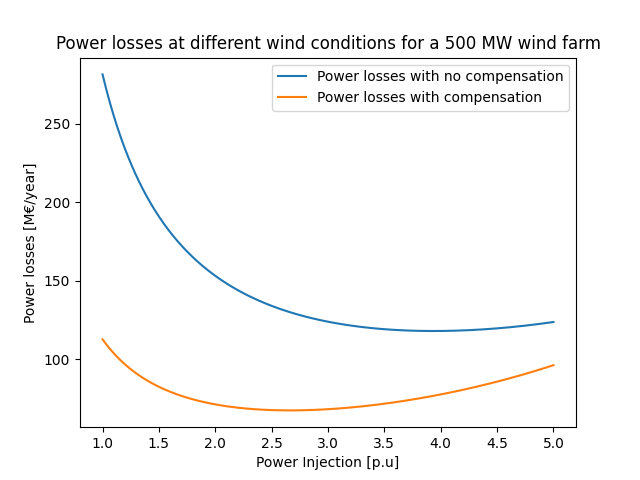
\includegraphics[width=0.65\textwidth]{imatges/why_compensation.png}
	\caption{Power losses comparison when including mid-cable reactive power compensation.}
	\label{fig:whycomp} %Si es posen les etiquetes de forma ordenada, la vida es més fàcil...
\end{figure}

The goal of the project is to determine where this compensation has to be placed  and how to size it. But this is only part of the design characteristics we want to optimize. A full description of the optimization variables will be
presented in Chapter \ref{Minimization}.

Taking all this into consideration, a HVAC transmission system layout for an OWPP with reactive power compensation looks like the one in Fig. \ref{fig:fulltransmission}.
\begin{figure}[H] %Recorda fixar la posició de les figures si no
    \centering
    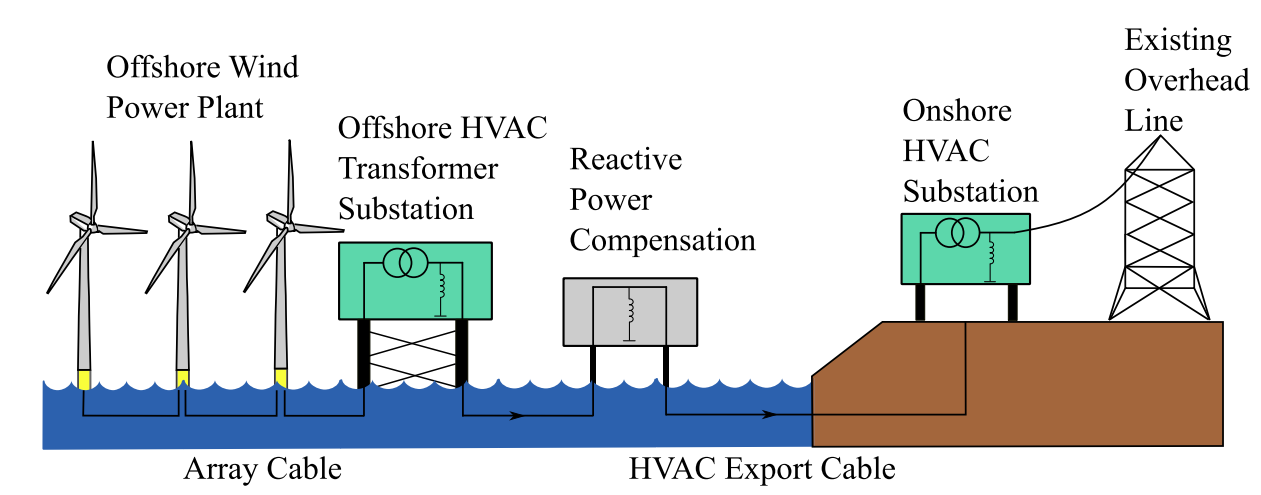
\includegraphics[width=0.75\textwidth]{imatges/layout.png}
    \caption{HVAC transmission system layout for an OWPP with reactive power compensation \cite{paperbase}.}
    \label{fig:fulltransmission} %Si es posen les etiquetes de forma ordenada, la vida es més fàcil...
\end{figure}

From this general layout we will be able to create the network model using the equivalent circuits of the  elements involved.

\subsection{Elements Modelling}\label{elementsmodelling}

To be able to do a steady-state analysis of the transmission system we need to model all the elements in the grid. This section models these elements and presents
some important concepts to understand the system.




\subsubsection{Cables}

Cables are an essential part of HVAC transmission systems, since they are in charge of transmitting the power from the OWPP to
shore and are the main source of active power losses and reactive power generation. We will consider  three-core cross-linked Polyethylene (XLPE) cables, which are the most common type of cables used in  AC OWPP's since they are
specifically designed for underwater applications, and they have lower dielectric losses than EPR (Ethylene Propylene Rubber) or fluid-filled cables \cite{ABB2}.  \par

Three-core XPLE cables (see Fig. \ref{fig:cableshape}) have a steel wire armour and can have either copper or aluminum as conductor. We will consider the cooper ones since they have higher current rating at the same cross-section \cite{ABB}. 

\begin{figure}[H]
    \centering
    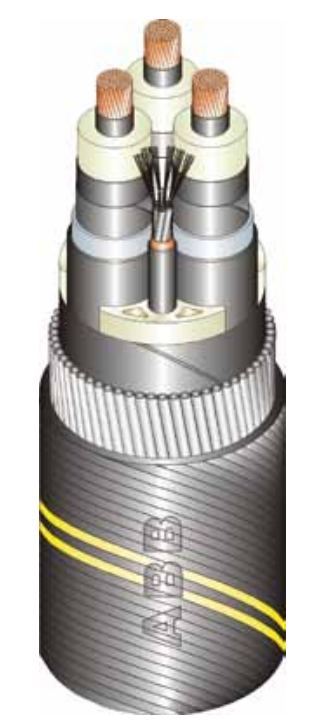
\includegraphics[width=0.15\textwidth]{imatges/cable shape.png}
    \caption{Three-core XLPE cable cross-section \cite{ABB}.}
	\label{fig:cableshape}
\end{figure}
Recall, as seen in \ref{tab:capacitance_comparison}, that the capacitance of underground cables is quite large, which leads to high reactive power generation. Reactive power compensation will
help us mitigate this effect.\par

For the equivalent circuit of a long transmission cables, we can use the following $\pi$-model, shown in Fig. \ref{fig:piline}.

\begin{figure}[h]
\centering
\begin{circuitikz}
    \draw (0,0) to [generic, l=$\underline{Z}_{\pi}$] (6,0);
    \draw (1,0) to [generic, l=$\underline{Y}_{\pi}$] (1,-2);
    \draw (5,0) to [generic, l=$\underline{Y}_{\pi}$] (5,-2);
    \draw (0,-2) -- (6,-2);
\end{circuitikz}
\caption{$\pi$-model transmission line.}
\label{fig:piline} 
\end{figure}   

We can use the following equations \cite{paperbase} to get the parameters:
\begin{align}
\begin{bmatrix}
\underline{V}_s \\
\underline{I}_s
\end{bmatrix}
&=
\begin{bmatrix}
\cosh(\underline{\theta}) & \underline{Z}_c \sinh(\underline{\theta}) \\
\frac{1}{\underline{Z}_c} \sinh(\underline{\theta}) & \cosh(\underline{\theta})
\end{bmatrix}
\begin{bmatrix}
\underline{V}_r \\
\underline{I}_r
\end{bmatrix} \\
\underline{Z}_c &= \sqrt{\frac{\underline{Z}}{\underline{Y}}}; \quad \underline{\theta} = l\sqrt{\underline{Z}\underline{Y}} \\
\underline{Z} &= R + j\omega L; \quad \underline{Y} = j\omega\frac{C}{2}
\end{align}

where $\underline{V}_s$ and $\underline{I}_s$ are the sending end voltage and current and $\underline{V}_r$ and $\underline{I}_r$ are the receiving end voltage and current,
$\underline{Z}_c$ is the characteristic impedance and $\underline{\theta}$ is the characteristic angle.
The parameters in Table \ref{tab:parameters} are obtained from manufacturer data \cite{ABB}.

%Afegir lo de R effects SI DONA TEMPSSSSSSSS i citar

\begin{table}[h]
\centering
\begin{tabular}{|c|c|}
\hline
Symbol & Description \\
\hline
$R \quad \left[\frac{\Omega}{\text{km}}\right]$  & Resistance per unit length \\
$L \quad \left[\frac{H}{\text{km}}\right]$ & Inductance per unit length \\
$C \quad \left[\frac{F}{\text{km}}\right]$ & Capacitance per unit length \\
\hline
\end{tabular}
\caption{Electrical parameters of AC cables.}
\label{tab:parameters}
\end{table} 



Therefore, the equivalent $\pi$ model is given by:
\begin{align}
\underline{Z}_{\pi} &= \underline{Z}_c \sinh(\underline{\theta}) = \underline{Z} l \frac{\sinh(\underline{\theta})}{\underline{\theta}} \\
\underline{Y}_{\pi} &= \frac{\tanh(\underline{\theta}/2)}{\underline{Z}_c} = \frac{\underline{Y} l}{2} \frac{\tanh(\underline{\theta}/2)}{\underline{\theta}/2}
\end{align}

%\newpage
\subsubsection{Transformers}
Transformers are essential devices in power transmission systems that transfer electrical energy between circuits through electromagnetic induction.
They enable voltage levels to be increased (stepped up) for efficient, long-distance transmission and decreased (stepped down) for safe distribution to homes and businesses.
This voltage transformation minimizes energy losses and enhances the stability of the power grid. Without transformers, the high currents required for low-voltage transmission would lead to excessive heat generation and energy losses,
reducing the efficiency and reliability of the electrical supply. Thus, transformers are crucial for optimizing power delivery and ensuring the safety and efficiency of electrical systems.

In our OWPP transmission system we will need to employ transformers to step up the voltage of the power generated by the wind turbines to the nominal voltage of the transmission system and another one at onshore to set
the voltage required by the main grid we are supplying to.

We will use the model in Fig. \ref{fig:transformer} to represent the transformer:
\begin{figure}[H]
\centering
\begin{circuitikz}
    \draw (0,0) to [generic, l=$\underline{Z}_{tr}$] (6,0);
    \draw (1,0) to [generic, l=$\underline{Y}_{tr}$] (1,-2);
    \draw (0,-2) -- (6,-2);
\end{circuitikz}
\caption{Transformer model.}
\label{fig:transformer}
\end{figure}

The equivalent impedance $\underline{Z}_{tr}$ and admittance $\underline{Y}_{tr}$ are given by \cite{paperbase}:
\begin{subequations}
\begin{align}
    \underline{Z}_{tr} &= R_{tr} + jX_{tr}; \quad
    \underline{Y}_{tr} = G_{tr} + jB_{tr} \\
    R_{tr} &= P_{Cu}^{loss} \left(\frac{U_{r-tr}}{S_{r-tr}}\right)^2 \quad
    X_{tr} = \sqrt{ \left(u_k\frac{U_{r-tr}}{S_{r-tr}}\right)^2 - R_{tr}^2} \\
    G_{tr} &= \frac{P_{Fe}^{loss}}{U_{r-tr}^2} \quad
    B_{tr} = i_o \frac{S_{r-tr}}{U_{r-tr}^2}
\end{align}
\end{subequations}

where $P_{Cu}^{loss}$ are the copper losses, $U_{r-tr}$ the rated  voltage of the transformer at the transmission system side, $S_{r-tr}$ the rated power of the transformer, 
$u_k$ the short-circuit voltage, $P_{Fe}^{loss}$ the iron losses and $i_o$ the open circuit current.


\subsubsection{Shunt Reactors: Reactive Power Compensation}
To compensate reactive power generation we will use shunt reactors. They are reactive power absorbers and in our case will be connected from
the line directly to the ground. The equivalent circuit is shown in Fig. \ref{fig:shuntreactor}.
\begin{equation}
    \underline{y}_{sh} = \frac{1}{j\omega L}
\end{equation}
where $L$ is the inductance of the reactor.
\begin{figure}[h]
\centering
\begin{circuitikz}
    \draw (0,0) to [generic, l=$\underline{y}_{sh}$] (0,-3) node[ground]{};
    
\end{circuitikz}
\caption{Shunt reactor model.}
\label{fig:shuntreactor}
\end{figure}

We will consider the possibility to include 5 different shunt reactors in the system. Further development on the reasoning of this scheme on Chapter \ref{fulltransmission}.

\subsubsection{Main Grid}
The main grid is the distribution grid we are supplying power to fit the OWPP.
We will model the grid we are connected to using a Thévenin equivalent circuit where $\underline{U}_{g}$ is the
Thévenin voltage and $\underline{Z}_{g}$ is the Thévenin impedance \cite{paperbase}:
\begin{figure}[H]
    \centering
    \begin{circuitikz}
        \draw (0,0) to[sV, l=$\underline{U}_{g}$] (0,-3) to (0,-3) node[ground]{};
        \draw (0,0) to [generic, l=$\underline{Z}_{g}$](-2,0);   
    \end{circuitikz}
    \caption{Main grid model.}
    \label{fig:maingrid}
    \end{figure}  
The equations describing the Thévenin equivalent circuit are:
\begin{subequations}\label{maingrideq}
\begin{align}
    \underline{Z}_{g} &= R_g + jX_g \\
    R_g &= \sqrt{\frac{\frac{U_{g}^2}{SCR} \, p_{owf}S_{base}}{(\frac{X_g}{R_g})^2+1}} \\
    X_g &= R_g \frac{X_g}{R_g}
\end{align}
\end{subequations}
where $U_{g}$ is the rated voltage of the grid, $SCR$ the short-circuit ratio and $\frac{X_g}{R_g}$ the ratio of the system reactance.
\begin{itemize}
    \item The $SCR$ is the ratio of the short circuit apparent power in the case of a balanced
    fault at the location in the grid where some generator is connected to the power rating of the generator itself.
    It is somehow a measure of the grid strength to changes in active and reactive power injections.
\end{itemize}


\subsubsection{Offshore Wind Power Plant}
We will model our OWPP as a simple power injection at one end of the transmission line. For our
analysis we will consider that there is no reactive power generation, therefore $q_{owf} = 0$. $p_{owf}$ will be the active power generation that will depend 
on the wind conditions of the plant. The reach of the work will limit its analysis to a fix power generation.
\begin{figure}[H]
\centering
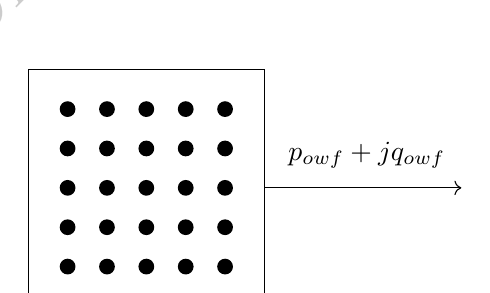
\begin{tikzpicture}
    \draw (0,0) rectangle (3,3);
    % Draw the dots
    \foreach \x in {0.5,1,1.5,2,2.5}
        \foreach \y in {0.5,1,1.5,2,2.5}
            \fill (\x,\y) circle (0.1);
    \draw[->] (3,1.5) -- (5.5,1.5);
    \node at (4.3,1.5)[label ={[font=\bfseries] above:$p_{owf}+jq_{owf}$}]{};
\end{tikzpicture}
\caption{ Offshore Wind Power Plant.}
\label{fig:powerplant}
\end{figure}
Further development on how considering different wind conditions could be implemented in our work, check section \ref{futurework}.


\subsection{Costs Modelling}

In this section we will derive the cost equations for the different elements of our transmission system. These costs function will be essential for our optimization problem since
they will be the objective function to minimize and the parameters on which the vector of decision variables we want to get will depend on.
\subsubsection{Cables}

Equations to describe AC cables costs are presented in \cite{chalmers} as:
\begin{align}
    C_{cables} &= n_{cables} (A + B \exp(\frac{CS_n}{10^8})) \cdot E_{\frac{eu}{sek}} \cdot \frac{1}{10^6} \quad \left[\frac{M\euro}{\text{km}}\right] \\
    S_n &= \sqrt{3}V_{rated}I_{rated} \quad \left[\text{VA}\right]
\end{align}

where $S_n$ is the rated power of the cable, $n_{cables}$ is the number of cables, $A$, $B$ and $C$ are parameters that depend on the rated voltage of the cable, $E_{\frac{eu}{sek}=0.087}$ is the exchange rate between Euros and SEK (Swedish Króna) and $V_{rated}$ and $I_{rated}$ are the rated voltage and current of the cable respectively.
The parameters $A$, $B$ and $C$ are shown in Table \ref{tab:parameterscab}:
\begin{table}[H]
    \centering
    \begin{tabular}{c|c|c|c}
    \hline
    \textbf{Rated Voltage (kV)} & \textbf{A [$10^6$]} & \textbf{B [$10^6$]} & \textbf{C} \\
    \hline
    132 & 1.971 & 0.209 & 1.66 \\
    220 & 3.181 & 0.11 & 1.16 \\
    \hline
    \end{tabular}
    \caption{Parameters A, B, C for different rated voltages \cite{chalmers}.}
    \label{tab:parameterscab}
    \end{table}
We will consider the transmission voltage levels presented in Table \ref{tab:parameterscab} as decision variables in our optimization.


\subsubsection{Transformers}
For the transformers, costs are defined in \cite{costraf} as:
\begin{equation}
    C_{tr}= 0.0427 \cdot S_{r-tr}^{0.7513} \quad \left[M\euro\right]
\end{equation}
where $S_{r-tr}$ is the rated power of the transformer in MVA.

\subsubsection{Shunt Reactors}
Cost functions for shunt reactors are presented in \cite{paperbase} as:
\begin{equation}\label{eq:shuntcost}
    C_{sh}= K \cdot Q_l \cdot + P = K \cdot Y_l\cdot U_{AC-N}^2 + P \quad \left[M\euro\right]
\end{equation}

where $K$ and $P$ are constants that depends on the location of the reactor and can be found in Fig. \ref{tab:parametersshunt}, $Q_l = Y_l\cdot U_{AC-N}^2$ is the reactive power absorbed by the reactor in MVAr,
$Y_l$ is the admittance of the reactor and $U_{AC-N}$ is the nominal transmission voltage where the compensation is placed.


\begin{table}[H]
    \centering
    \begin{tabular}{c|c|c}
    \hline
    \textbf{Location} & \textbf{K} & \textbf{P} \\
    \hline
    Onshore & 0.01049 & 0.8312  \\
    Offshore & 0.01576 & 1.244 \\
    Mid-cable & 0.01576 & 12.44 \\
    \hline
    \end{tabular}
    \caption{Parameters K and P for different positions of the reactive power compensation \cite{paperbase}.}
    \label{tab:parametersshunt}
    \end{table}
\subsubsection{Switchgears}

For switchears, costs are defined in \cite{switchcost} as:
\begin{equation}
    C_{gis-AC} = 0.0117 \cdot U_{AC-N} + 0.0231 \quad \left[M\euro\right]
\end{equation}

where $U_{AC-N}$ is the nominal transmission voltage in kV.
\subsubsection{Substation Platform}
For the substation platform, costs are presented in \cite{chalmers} as:
\begin{equation}
    C_{ss-AC} = 2.534 + 0.0887 \cdot P_{owf} \quad \left[M\euro\right]
\end{equation}
where $P_{owf}$ is the nominal power generated by the OWPP in MW.

\subsubsection{AC Power Losses}
Lastly, but probably one of the most important costs to consider, are the power losses in the transmission system. To be able to compare this term with other investment costs related to the electric elements,
it would be useful to express this term in monetary units. We will use the following equation to estimate the cost of power losses in the system:

\begin{equation}\label{eq:lossescost}
    C_{loss-AC} = 8760 \cdot t_{owf} \cdot C_{energy} \cdot P_{loss} \cdot 10^{-6} \quad \left[M\euro\right]
\end{equation}
where $8760$ is the number of operating hours in a year, $t_{owf}$ is the expected lifetime of the OWPP in years, $C_{energy}$ is the cost of energy in \euro/MWh and $P_{loss}$ is the power losses in the system in MW. We will be using the
following estimated values from \cite{paperbase}:
\begin{table}[h]
    \centering
    \begin{tabular}{c|c}
    \hline
    \textbf{Parameter} & \textbf{Value} \\
    \hline
    $t_{owf}$ & 30 years \\ 
    $C_{energy}$ & 100 \euro/MWh  \\
    \hline
    \end{tabular}
    \caption{Parameters for computing power losses cost \cite{paperbase}.}
    \label{tab:lossescost}
\end{table}

Now it remains to compute the power losses $P_{losses}$ in the system. This will be derived in section \ref{fulltransmission} as it will be trivial to get
the power losses once we have the power flow solution.

\section{Power Flow Analysis} \label{fulltransmission}

Now we can fully define the power flow analysis.  This approach will allow as to model the transmission system as a set of buses (or nodes)
interconnected by transmission links. It will allow as to solve for the steady-state powers and voltages of the system. This step is crucial to latter on
formulate our optimization since power flow equations will be the equality constraint of the optimization problem,  see section \ref{equality}, and the objective function will also depend on the solution of the power flow (PF).

\subsection{Types of Buses}

In this section we will briefly describe what is a bus and what types we have.\par
Buses are points of the grid which either supplied by generators, \textit{generator buses}, or those without generators, \textit{load buses}. More formally, an $n$-bus system, $N=\{B_1,...,B_i,...,B_n\}$ where $N$ is the set of $n$-nodes, is defined as:

\begin{equation}
    \forall B_i \in N,
    \begin{cases}
        S_i = P_i + jQ_i, & \text{where } S_i \text{ is the apparent power at bus } i \\
        V_i = |V_i|e^{j\theta_i}, & \text{where } V_i \text{ is the complex voltage at bus } i
    \end{cases}
    %\forall i \in N,  \text{where } N={1,2,...,i,...,n}
\end{equation}

As we can see, for each bus $i$ we have 4 variables:

\begin{itemize}
    \item $P_i$ and $Q_i$ are the active and reactive power at bus $i$ respectively.
    \item $|V_i|$ and $\theta_i$ are the voltage magnitude and angle at bus $i$ respectively.
\end{itemize}

It is important to note that in general we cannot specify all the $P_i$'s independently since there is a constraint imposed by the need to balance active power. In our case, a transmission system with losses, which are unknown before the PF,
the sum of $P_i$'s must be equal to losses. To tackle this we will define one bus as the $slack$ bus, where power injection is left free. Taking all of this account, depending on the variables are known and unknown for a certain bus we can classify them as:
\begin{itemize}
    \item \textbf{Slack bus:} The slack bus is the reference bus of the system. It is the bus where the voltage magnitude and angle are known, typically $|V_i|= 1, \theta_i= 0 $.
    All other buses angles will be referenced to the $slack$. It is used to balance the active and reactive power in the system.
    \item \textbf{Generator bus (PV):} The generator bus is the bus where the active power and voltage are known.
    \item \textbf{Load bus (PQ):} The load bus is the bus where the active and reactive power are known. The voltage magnitude and angle are unknown.
\end{itemize}
In summary:
\begin{table}[h]
    \centering
    \begin{tabular}{|c|c|c|c|}
        \hline
        & Slack Bus & PQ & PV \\
        \hline
        Voltage Magnitude ($|V_i|$) & Yes & No & Yes \\
        \hline
        Voltage Angle ($\theta_i$) & Yes & No & No \\
        \hline
        Active Power ($P_i$) & No & Yes & Yes \\
        \hline
        Reactive Power ($Q_i$) & No & Yes & No \\
        \hline
    \end{tabular}
    \caption{Known variables for each type of bus.}
    \label{tab:bus_variables}
\end{table}





\subsection{Per-Unit System (p.u.)}

In power systems analysis, it is common to use the per-unit system to normalize the magnitudes of the variables. This is very useful when we are dealing with several transformers and voltage levels. 
The per-unit system is defined as:
\begin{equation}
    \text{Per unit value} = \frac{\text{Actual value}}{\text{Base value}}
\end{equation}

In our case we will use $S_{base} =100 \text{ MVA}$ and $V_{base} = \text{ transmission voltage in kV}$ as the base values. This means that the per-unit system will be defined as:
\begin{equation}
    \begin{cases}
        I_{base} = S_{base}V_{base} \\
        Y_{base} = \frac{S_{base}}{V_{base}^2} \\
    \end{cases}
\end{equation}

Using the per-unit system will be particularly useful for analyzing the results and for dealing with the inequality constraints in section \ref{inequality}.

\subsection{Full Transmission System Model}

Now we have all the information needed to build our full model. In \cite{paperbase} they consider five possible positions for the shunt reactors, as seen in Fig. \ref{fig:poss_position}. 
\begin{figure}[H]
    \centering
	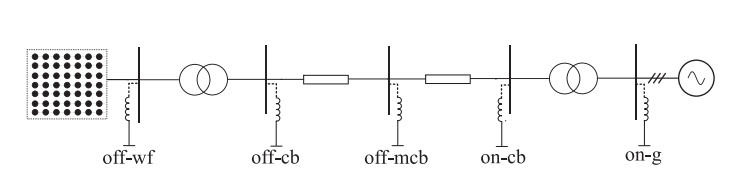
\includegraphics[width=0.65\textwidth]{imatges/poss_position.png}
	\caption{Possible locations for the shunt reactors \cite{paperbase}.}
    \label{fig:poss_position}
\end{figure}



They consider when optimizing the cost function only the combinations where: if at a given transformer you place a reactor before it, you won't consider placing another one
after the same transformer. For sake of generality, we will consider that any combination within the five possible positions is valid. This will lead to a total of $2^5 = 32$ possible combinations.




\begin{figure}[h]
    \centering
    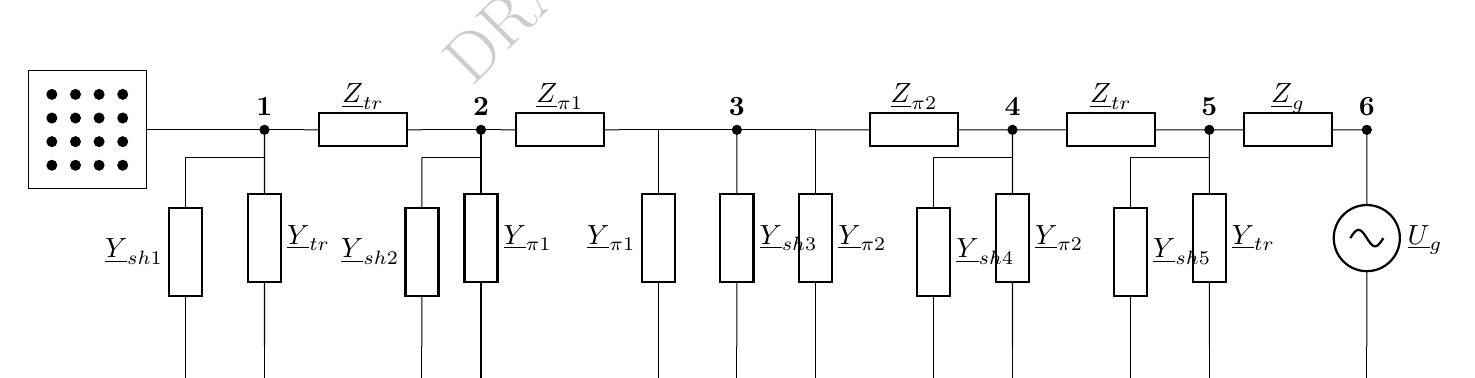
\begin{tikzpicture}[scale=1]
        \draw (0,0) rectangle (1.5,1.5);
        % Draw the dots
        \foreach \x in {0.3,0.6,0.9,1.2}
            \foreach \y in {0.3,0.6,0.9,1.2}
                \fill (\x,\y) circle (0.07);
        
        \draw (1.5,0.75) -- (3.5,0.75);
        \node at (3,0.75) [circle, draw=black, fill=black, inner sep=1pt, thick, label=above:$\textbf{1}$]{};
        \draw (3.5,0.75) to [generic, l=$\underline{Z}_{tr}$] (5,0.75);
        \draw (3,0.75) to [generic, l=$\underline{Y}_{tr}$] (3,-2) node[ground]{};
        \draw (3,0.4) -- (2,0.4);
        \draw (2,0.4) to [generic, l_=$\underline{Y}_{sh1}$] (2,-2)node[ground]{};
        \draw (5,0.75) -- (6,0.75);
        \node at (5.75,0.75) [circle, draw=black, fill=black, inner sep=1pt, thick, label=above:$\textbf{2}$]{};
        \draw (6,0.75) to [generic, l=$\underline{Z}_{\pi1}$] (7.5,0.75);
        \draw (5.75,0.75) to [generic, l=$\underline{Y}_{\pi1}$] (5.75,-2) node[ground]{};
        \draw (5.75,0.4) -- (5,0.4);
        \draw (5,0.4) to [generic, l_=$\underline{Y}_{sh2}$] (5,-2)node[ground]{};
        \draw (7.5,0.75) -- (10,0.75);
        \node at (9,0.75) [circle, draw=black, fill=black, inner sep=1pt, thick, label=above:$\textbf{3}$]{};
        \draw (8,0.75) to [generic, l_=$\underline{Y}_{\pi1}$] (8,-2) node[ground]{};
        \draw (9,0.75) to [generic, l^=$\underline{Y}_{sh3}$] (9,-2) node[ground]{};
        \draw (10,0.75) to [generic, l=$\underline{Y}_{\pi2}$] (10,-2)node[ground]{};
        \draw (10,0.75) to [generic, l=$\underline{Z}_{\pi2}$] (12.5,0.75);
        \draw (12.5,0.75) to [generic, l=$\underline{Y}_{\pi2}$] (12.5,-2) node[ground]{};
        \draw (12.5,0.4) -- (11.5,0.4);
        \node at (12.5,0.75) [circle, draw=black, fill=black, inner sep=1pt, thick, label=above:$\textbf{4}$]{};
        \draw (11.5,0.4) to [generic, l=$\underline{Y}_{sh4}$] (11.5,-2)node[ground]{};
        \draw (12.5,0.75) to [generic, l=$\underline{Z}_{tr}$] (15,0.75);
        \draw (15,0.75) to [generic, l=$\underline{Y}_{tr}$] (15,-2) node[ground]{};
        \node at (15,0.75) [circle, draw=black, fill=black, inner sep=1pt, thick, label=above:$\textbf{5}$]{};
        \draw (15,0.4) -- (14,0.4);
        \draw (14,0.4) to [generic, l=$\underline{Y}_{sh5}$] (14,-2) node[ground]{};
        \draw (15,0.75) to [generic, l=$\underline{Z}_{g}$](17,0.75);
        \draw (17,0.75) to[sV, l=$\underline{U}_{g}$] (17,-2) to (17,-2) node[ground]{};
        \node at (17,0.75) [circle, draw=black, fill=black, inner sep=1pt, thick, label=above:$\textbf{6}$]{};
    

    \end{tikzpicture}
    \caption{Transmission system model and buses.}
    \label{fig:fullgrid}
    \end{figure}

Now we choose where we want to define our buses and which type they are. We classify them as in Table \ref{table:bus_types}.
\begin{table}[h]
\centering
\begin{tabular}{c|c}
\hline
\textbf{Bus Number} & \textbf{Bus Type} \\
\hline
1 & PQ \\
2 & PQ \\
3 & PQ \\
4 & PQ \\
5 & PQ \\
6 & Slack \\
\hline
\end{tabular}
\caption{Transmission system bus types.}
\label{table:bus_types}
\end{table}

A brief explanation of the bus types is exposed:
\begin{itemize}
    \item \textbf{Bus 1:} It is the bus where the OWPP is injecting power therefore active and reactive power are specified as $P_1=p_{owf}$ and $Q_1=q_{owf}$.
    \item \textbf{Bus 2, 3, 4, 5:} Those buses are plain  PQ load buses, where $P_i=0, Q_i=0$. We want to consider them as we will be interested in the voltage levels in the lines in order
    to compute possible over and undervoltages in the cables, as we will see in Chapter \ref{Minimization}.
    \item \textbf{Bus 6:} We will use this one as the slack bus. Note that this bus power flow solution for $P_6$ will allow us to compute the losses in the system
    and will be essential part of the optimization problem. Also, since we define it as the slack bus, it will be the reference for the voltage angles and in charge of balancing the power in the transmission system. 
\end{itemize}
\subsection{Admittance Matrix}

The admittance matrix encodes all the information of the passive elements of the grid and the relationship between them and allows us to perform the steady-state 
analysis of the grid.
Now we can build the full HVAC transmission system model and fins its admittance matrix $\underline{Y}_{bus}$, which will be essential
for the power flow solver.

Inspecting the Kirchhoff's Current Law (KCL) we can observe how the admittance matrix is the fundamental relationship between voltages and currents :
\begin{equation}
\textbf{I} = \textbf{Y}_{bus} \textbf{V}
\label{eq:kirchhoff}
\end{equation}

where $\textbf{I}$ is the vector of injected currents, $\textbf{Y}_{bus}$ is the admittance matrix and $\textbf{V}$ is the vector of bus voltages.

Since we will be using the per-unit system:
\begin{equation}
    y_i = \frac{Y_i}{Y_{base}}
\end{equation}

Note that when we build $\textbf{Y}_{bus}$ , we take the series impedance in Eq. \ref{fig:fullgrid}, compute their inverse and add the sub-index $s$ to identify them. For example:
\begin{equation}
    \underline{y}_{\pi1s} = \frac{1}{\underline{z}_{\pi1}}
\end{equation}

%We build $\underline{Y}_{bus}$ by inspection 

    
\begin{equation} \label{ybus}
    \resizebox{0.92\textwidth}{!}{%
    $\mathbf{{Y}_{bus}}=\begin{bmatrix}
        (\underline{y}_{tr}+\underline{y}_{trs}+\underline{y}_{sh1}) & -\underline{y}_{trs} & 0 & 0 & 0 & 0\\
       -\underline{y}_{trs} & (\underline{y}_{\pi1}+\underline{y}_{\pi1s}+\underline{y}_{sh2}+\underline{y}_{trs}) & -\underline{y}_{\pi1s} & 0 & 0 & 0  \\
       0 & -\underline{y}_{\pi1s} & (2\underline{y}_{\pi1}+2\underline{y}_{\pi1s}+\underline{y}_{sh3}) & -\underline{y}_{\pi2s}   & 0 & 0 \\
       0 & 0 & -\underline{y}_{\pi2s} & (\underline{y}_{\pi2}+\underline{y}_{\pi2s}+\underline{y}_{sh4}+\underline{y}_{trs}) & -\underline{y}_{trs} & 0  \\
       0 & 0 & 0 & -\underline{y}_{trs} & (\underline{y}_{tr}+\underline{y}_{tr}+\underline{y}_{sh5}+\underline{y}_{g}) & -\underline{y}_{g}  \\
       0 & 0 & 0 & 0 & -\underline{y}_{g} & \underline{y}_{g}\\
       \end{bmatrix}$
    }
\end{equation}

Some properties of the admittance matrix are:
\begin{itemize}[itemsep=0pt]
    \item It is a square matrix of size $n \times n$, where $n$ is the number of buses in the system.
    \item It is symmetric. Note that this condition does not hold for certain types of transformers.
    \item The diagonal elements, $Y_{ii}$, are self-admittance, equal to the sum of the admittances of elements connected to bus $i$. Note that this condition does not hold for certain types of transformers.
    \item $Y_{ij}$ is the negative of the admittance between buses $i$ and $j$.
    \item  For our system, the sparcity is $\frac{20}{36}= 56\%$. Nevertheless, for large networks, the matrix is very sparse. The level of sparsity, which is the percentage of zero elements in a matrix, increases with the size of the network.
    For instance, in a 1000-bus system, the matrix approximately is 99\% sparse. You can take advantage (and it will be essential to do it for very big networks) of this sparsity using computational techniques \cite{sparcity}.
\end{itemize}

\subsection{Transmission System Parameters}

We will use the following set of grid elements parameters for the transformers and the main grid:
\begin{table}[h]
    \centering
    \renewcommand{\arraystretch}{1.2}
    \begin{tabular}{l|c}
    \hline
    \textbf{Parameter} & \textbf{Value} \\
    \hline
    $SCR$ & \ 5 \\
    $\frac{X_g}{R_g}$ & 10 \\
    $P_{Cu}^{loss}$ & 60 kW \\
    $P_{Fe}^{loss}$ & 40 kW \\
    $u_k$ & 18 \%  \\
    $i_o$ & 1.2 \% \\
    \hline
    \end{tabular}
    \caption{Grid parameters \cite{paperbase}.}
    \label{tab:gridparameters}
    \end{table}


\subsection{Power Flow }
\subsubsection{Power Flow Equations}

We are first going to derive an expression for the PF equations.
From Eq. \ref{eq:kirchhoff} we can get the injected current for the $i$-th component:
\begin{equation}
    I_i = \sum_{j=1}^{n} Y_{ik}V_k \quad i = 1,2,...,n
\end{equation}
Now we can compute the $i$-th bus power:
\begin{equation}
    S_i = V_iI_i^* = V_i\sum_{k=1}^{n} Y_{ik}^*V_k^* \quad i = 1,2,...,n
\end{equation}

Now if we let $V_i = |V_i|e^{j\theta_i}$, and $Y_{ik} = G_{ik} + jB_{ik}$, we can write the power at bus $i$ as:
\begin{equation}
    S_i = \sum_{k=1}^n|V_i||V_k|e^{j\theta_i}(G_{ik} - jB_{ik}) = \sum_{k=1}^n|V_i||V_k|(cos(\theta_{ik})+jsin(\theta_{ik}))(G_{ik} - jB_{ik}) \quad i = 1,2,...,n
\end{equation}

Note that the real part of the admittance, $G_{ik}$, is the conductance and the imaginary part, $B_{ik}$, is the susceptance. Now if we separate the real and imaginary parts of the power we get:

\begin{align}
    P_i= \sum_{k=1}^n|V_i||V_k|(G_{ik}cos(\theta_{ik}) + B_{ik}sin(\theta_{ik}))\label{powerflowP} \quad i= 1,2,...,n \\
    Q_i= \sum_{k=1}^n|V_i||V_k|(G_{ik}sin(\theta_{ik}) - B_{ik}cos(\theta_{ik}))\label{powerflowQ} \quad i= 1,2,...,n
\end{align}  


\subsubsection{Newton-Raphson Solver}\label{NRsolver}

\paragraph{Problem Solvability}

First, we have to make sure that our set of equations is solvable. If we strip away the $slack$-bus, we have 5 $PQ$-buses remaining. Each $PQ$-bus introduces 2 unknowns, $|V_i|$ and $\theta_i$, and 2 equations, $P_i$ and $Q_i$. This means that we have 10 equations and 10 unknowns. 
After solving the system, from  Eq. \ref{powerflowP} and Eq. \ref{powerflowQ} we can solve for the power injections of the slack bus, $P_6$ and $Q_6$. Hence, the condition for solvability is fulfilled.

To solve a set of non-linear equations, numerical methods are the standalone way to go. For the PF, one of the most used methods is the Newton-Raphson (N-R) method \cite{NRusual}. A brief description of this method will be presented for the $n$-dimentional case, but further description can be found in \cite{llibrebase}.

We will describe the process considering an $n$-bus system with all PQ buses except one slack bus. Note that in our specific case these conditions are met and $n = 6$. Once we strip away the slack bus, it remains to find the unknowns on the right side of Eqs. \ref{powerflowP} and \ref{powerflowQ}. Therefore, it will be convenient to
define the following vectors of unknowns of PQ-buses:
\begin{equation}
\begin{aligned}
    \mathbf{\theta} &= \begin{bmatrix}
    \theta_1 \\
    \theta_2 \\
    \vdots \\
    \theta_{n-1}
    \end{bmatrix} &
    \mathbf{|V|} &= \begin{bmatrix}
    |V_1| \\
    |V_2| \\
    \vdots \\
    |V_{n-1}|
    \end{bmatrix} &
    \mathbf{x} &= \begin{bmatrix}
    \mathbf{\theta} \\
    \mathbf{|V|} \\
    \end{bmatrix}
\end{aligned}
\end{equation}

Now the dependency between the power flow equations and the vector of unknowns $\mathbf{x}$ can be easily shown:
\begin{subequations}
\begin{align}
    P_i = P_i(\mathbf{x}) \quad i = 1,2,...,n-1 \\
    Q_i = Q_i(\mathbf{x}) \quad i = 1,2,...,n-1
\end{align}       
\end{subequations}

The N-R method is an iterative method that starts with an initial guess of the unknowns, $\mathbf{x}_0$, and then iterates the vector $\mathbf{x}$ until the right side matches the left side of the equations. Therefore, we
can define the power mismatch vector $\mathbf{f(x)}$ as:
\begin{equation}
\begin{aligned}
    \mathbf{f(x)} = \begin{bmatrix}
    P_1(\mathbf{x}) - P_1 \\
    \vdots \\
    P_{n-1}(\mathbf{x}) - P_{n-1} \\
    Q_1(\mathbf{x}) - Q_1 \\
    \vdots \\
    Q_{n-1}(\mathbf{x}) - Q_{n-1}
    \end{bmatrix} = \begin{bmatrix}
    \mathbf{\Delta P(\mathbf{x})} \\
    \mathbf{\Delta Q(\mathbf{x})}
    \end{bmatrix} = \mathbf{0}
\end{aligned}
\label{powermismatch}
\end{equation}


Now we have to consider $\mathbf{J}$, the Jacobian matrix of $\mathbf{f(x)}$. For clarity, is convenient to partition $\mathbf{J}$ as:
\begin{equation}
\begin{aligned}
    \mathbf{J} = \begin{bmatrix}
    \mathbf{J_{11}} & \mathbf{J_{12}} \\
    \mathbf{J_{21}} & \mathbf{J_{22}}
    \end{bmatrix} = \begin{bmatrix}
        \frac{\partial \mathbf{\Delta P}}{\partial \mathbf{\theta}} & \frac{\partial \mathbf{\Delta P}}{\partial \mathbf{|V|}} \\
        \frac{\partial \mathbf{\Delta Q}}{\partial \mathbf{\theta}} & \frac{\partial \mathbf{\Delta Q}}{\partial \mathbf{|V|}}
    \end{bmatrix} = \begin{bmatrix}
    \frac{\partial \mathbf{P}}{\partial \mathbf{\theta}} & \frac{\partial \mathbf{P}}{\partial \mathbf{|V|}} \\
    \frac{\partial \mathbf{Q}}{\partial \mathbf{\theta}} & \frac{\partial \mathbf{Q}}{\partial \mathbf{|V|}}
    \end{bmatrix}
\end{aligned}
\end{equation}

If interested, check derivation of the partial derivatives of the power flow equations with respect to the unknowns check the \hyperref[Appendix]{Appendix} or \cite{llibrebase}.

Now it just remains to find the step $\Delta \mathbf{x^k}$ to update $\mathbf{x}$ solving the following linear system by Gauss elimination:
\begin{equation}
    \mathbf{J^k}\Delta \mathbf{x^k} = -\mathbf{f(x^k)}
\end{equation}

Now we update $\mathbf{x^{k+1}}=\mathbf{x^{k}}+\Delta \mathbf{x^k}$ and iterate until it converges. The convergence criteria will be usually set as the maximum of the absolute value of the power mismatch vector, $\max(\mathbf{f(x)})$, is less than a tolerance, $tol$, 
which we have set to $10^{-6}$.







The N-R solver has been implemented in Python(check the \hyperref[Appendix]{Appendix}) and the procedure can be found in Algorithm 1.
\begin{algorithm}[H]
    \caption{Newton-Raphson Method}
    %\begin{algorithmic}[1]
    \begin{algorithmic}
    \Procedure{run\_pf}{}
        \State Initialize $V$ with ones and $\theta$ with zeros
        \Statex \hspace{\algorithmicindent}Set $V[slack$] to $1$, $\theta[slack]$ to $0$
        \Statex \hspace{\algorithmicindent}Set $P_{}$, $Q_{}$ based on OWPP data
        \Statex \hspace{\algorithmicindent}Set $iter = 0 $, $tol$ and $k = 0$
        \While{$iter$ < $max\_iter$ and $ \Delta PQ > tol$}
            \State Compute $P\_present$, $Q\_present$ using $V$, $\theta$, $Y_{bus}$
            \State Compute mismatch $\Delta PQ = [dP, dQ]$ as difference between calculated and given $P$, $Q$
            \State Compute the Jacobian matrix $J$.
            \State Solve the linear system $J \cdot \Delta x_k = -\Delta PQ$.
            \State Compute the updated $x^{k+1} = x^{k} + \Delta x^k $.
            \State Update $V$, $\theta$ using $dP$, $dQ$, $Y\_bus$
            \If{$\max(\Delta PQ) < tol$}
                %\State Converged
                \State \textbf{break}
            \EndIf
            
        \EndWhile
        \State \textbf{return} $V$, $\theta$
        \State Compute $P_{slack}$, $Q_{slack}$
    \EndProcedure
    \end{algorithmic}
    \end{algorithm}

Finally, note that close to the solution vector $\mathbf{x^{*}}$ it can be proven that N-R normally presents
quadratic convergence \cite{convergenceNR}. Moreover, in terms of computational time, Algorithm 1 takes about $0.06$ s in average to solve the PF.

Now we can observe that the PF is essential for computing the power losses (see Eq. \ref{eq:lossescost}) in the system, which will be in the objective function of the optimization problem. It is clear to see that $P_{losses}$ will be the difference between
the injected  active power from the OWPP and the active power delivered to the slack bus, which is the main grid:

\begin{equation}
    P_{losses} = (P_{owf} - P_{6}) \cdot S_{base} \cdot 10^{-6} \quad \text{MW}
\end{equation}


\section{Optimization Problem Formulation}\label{Minimization}

Generally an optimization problem that involves equality and inequality constraints can be formulated as:
\begin{equation}\label{optiprob}
    \begin{aligned}
        \text{min} \quad & \mathbf{f}(\mathbf{x})=(f_1(x),f_2(x),...,,f_k(x)) \\
        \text{subject to} \quad & \mathbf{H(x)} = 0 \\
        & \mathbf{G(x)} \leq 0
    \end{aligned}
\end{equation}


where $\mathbf{x} \in \mathbb{R}^n$ is the $n$ decision variables vector, $\mathbf{f}(\mathbf{x}) \in \mathbb{R}^k $ is set of objective functions to be minimized. Note we have presented the problem in its more general form, where the objective function can be a set of $n$-objectives to have to be optimized simultaneously and will
be proved to be useful in section \ref{objfun}. $\mathbf{H(x) = 0}$ are the equality constraints and $\mathbf{G(x) \leq 0}$ are the inequality constraints. 


Now we have to decide which decision variables we include in the optimization problem. It is easy to see that we can include all the design variables in which the transmission system model depends, which are all included
in the cost function and therefore have a direct impact in the cost of the system. By checking the parameters on which the admittance matrix depends, which can be found in section \ref{Grid}, we can define the vector of unknowns as:
\begin{equation}\label{vecunk}
    \resizebox{0.9\textwidth}{!}{%
    $\mathbf{x} = 
    \begin{bmatrix}
    vol_{tr}, & n_{cables}, & react_{bi_1}, &, ... &, react_{bi5}&, react_{cont1}&, ... &,react_{cont5}&, react_{bi5}&, S_{trafo}  
    \end{bmatrix}$
    }
\end{equation}

where the size of $\mathbf{x}$ is ($1$ x $13$), i.e. we have 13 decision variables. Each term is defined as follows:
\begin{itemize}
    \item $vol_{tr}$: Is the voltage level of the transmission cables. Note that this will be an integer variable, where you can choose one voltage level
    given by manufacturers with its associated parameters and cost. Check Table \ref{tab:parameterscab} to see available options considered.
    \item $n_{cables}$: Is an integer number that that represents the number of cables placed in parallel.
    \item $react_{bi_i} \quad i=1,...,5$: Is a binary variable (i.e. either 0 or 1) that tells if we place or not a reactor at position $i$.
    \item $react_{cont_i} \quad i=1,...,5$: Sizing of reactor at position $i$, therefore its $Y_{shi}$ in p.u.
    \item $S_{trafo}$: Rated power of the transformer in VA.
\end{itemize}

A very important remark with respect to the type of variables we have involved in the problem. Considering $\mathbf{x}$ we see that we have 
binary, integer and continuous variables. This kind of problems are labeled as mixed-variable optimization and constraints the optimization 
methods we can use as we will see in \ref{Optimization}.


\subsection{Constraints}
\subsubsection{Equality: Power Flow}\label{equality}

The equality constraints $ \mathbf{H(x)} = 0$ in the optimization problem in  Eq. \ref{optiprob} are the imposed by the power flow equations. In fact, the power mismatch vector in Eq. \ref{powermismatch} is the one that take this form. Therefore:

\begin{equation}
    \mathbf{H(x)} = \begin{bmatrix}
    \mathbf{\Delta P(\mathbf{x})} \\
    \mathbf{\Delta Q(\mathbf{x})}
    \end{bmatrix} = \begin{bmatrix}
    P_1(\mathbf{x}) - P_1 \\
    \vdots \\
    P_{n-1}(\mathbf{x}) - P_{n-1} \\
    Q_1(\mathbf{x}) - Q_1 \\
    \vdots \\
    Q_{n-1}(\mathbf{x}) - Q_{n-1}
    \end{bmatrix} = \mathbf{0}
\end{equation}



%Now we define de equality constraints as seen in  Eq. \ref{eqconstr}
%\begin{gather}
%    \mathbf{h_m(x) = 0 } \label{eqconstr} \\
%    \mathbf{S_i} = \mathbf{V_i(\sum_{j=1}^{N_{nodes}}Y_{ij}V_j)^*} \\
 %   \underline{s}_1-(p_{owf}+jq_{owf}) = 0, \nonumber \\
%  \underline{s}_1-\underline{u}_1[(2\underline{y}_{tr}+\underline{y}_l)\underline{u}_1-(\underline{y}_{tr})\underline{u}_2]^* = 0, \nonumber \\
 %   \underline{s}_2-\underline{u}_2[-(\underline{y}_{tr})\underline{u}_1+(2\underline{y}_{\pi1}+\underline{y}_l+\underline{y}_{tr})\underline{u}_2-(\underline{y}_{\pi1})\underline{u}_3]^* = 0, \nonumber \\
 %   \underline{s}_3-\underline{u}_3[-(\underline{y}_{\pi1})\underline{u}_2+(2\underline{y}_{\pi1}+2\underline{y}_{\pi2}+\underline{y}_{l})\underline{u}_3-(\underline{y}_{\pi2})\underline{u}_4]^* = 0, \nonumber \\
  %  \underline{s}_4-\underline{u}_4[-(\underline{y}_{\pi2})\underline{u}_3+(2\underline{y}_{\pi2}+\underline{y}_l+\underline{y}_{tr})\underline{u}_4-(\underline{y}_{tr})\underline{u}_5]^* = 0, \nonumber \\
   % \underline{s}_5-\underline{u}_5[-(\underline{y}_{tr})\underline{u}_4+(2\underline{y}_{tr}+\underline{y}_l+\underline{y}_{g})\underline{u}_5]^* = 0
%\end{gather}




\subsubsection{Inequality: Technical Constraints}\label{inequality}

The operational constraints are the ones that ensure the system operates within the limits of the equipment. These constraints of inequality nature, setting 
upper and lower bounds for certain variables. They will be the inequality constraints $\mathbf{G(x)} \leq 0$ in the optimization problem in  Eq. \ref{optiprob}. We will
denote as $\mathbf{L_i^X}$ each different limit at bus $i$ and for the sake of coherence we will express the constraints in the $\mathbf{G(x)} \leq 0$ form.\par
Note that all the following limits can be based on grid code requirements, but we will use some standard values.

\textbf{Bus voltage limits}\\
We set the nodal bus-$i$ voltage, $V_i$, limits as:
\begin{equation}
\begin{aligned}
    L_{i}^{Vu} &= V_i - V_{max} \leq 0, \quad i \in N \quad \text{is the upper limit} \\
    L_{i}^{Vl} &= V_{min} - V_i \leq 0, \quad i \in N \quad \text{is the lower limit}   
\end{aligned}    
\end{equation}

where $\mathbf{V_{max}}$ and $\mathbf{V_{min}}$ are the maximum and minimum voltages. These values have been taken to be $\pm 0.1$ p.u. of the nominal voltage respectively.

\textbf{Maximum current limits for the lines}\\
The current in the lines should not exceed the maximum current that the cables and transformers can handle. We will set $I_{max} = 1.1$ p.u. of the rated current of the cable $I_{rated}$. This rated current is given by manufacturers \cite{ABB}.
Therefore, the constraint will be:
\begin{equation}
    L_{i}^{I} = I_i - I_{max} \leq 0, \quad i \in N_{lines}
\end{equation}

\textbf{Reactive power delivered to the grid}\\
In general reactive power delivered to the grid, $Q_6$ can be defined by grid code requirements. Nevertheless, in this work we will aim to keep it as close as
possible to zero. Therefore, we will set the limits as:
\begin{equation}
\begin{aligned}
    L_{6}^{Qu} = Q_6 - Q_{max} \leq 0 \\
    L_{6}^{Ql} = Q_{min} - Q_{6} \leq 0
\end{aligned}
\end{equation}
where $Q_{max}=Q_{min}=0$. Also note that potentially the wind turbines could be used to absorb reactive power, but we will not consider this option in our work.


\subsection{Objective Function}\label{objfun}

Probably one of the critical parts is to identify the objective function we want to minimize and decide how we treat it. Now, we will describe the terms that we will include in the objective function
and why we have decided to work with a multi-objective approach.\par

\subsubsection{Why Bi-objective?} \label{biobjective}

Let us imagine you are an engineer of a firm that is planning to build and OWPP. You have to ensure both that the transmission system is reliable and robust in terms of operational constraints but also to make the
investment as profitable as possible, therefore you want to minimize its investment cost. Given this scenario, you can expect that it exists a trade off between the two objectives, investing more money can make your transmission system more robust and yield smaller power losses and
vice versa. In fact, in eRoots project for Acciona, they have shown interest on getting insights on how these two objectives interact with them and decide which option to go for given the relationship.\par

Literature can offer solutions for this kind of scenarios. Multi-objective optimization, also known as Pareto optimization, deals with situations where optimal decision-making
needs to be taken in presence of various conflicting objectives.  Within this context, there is no guarantee that there exist a unique solution that minimizes both objectives.
The main idea is to find the set of solutions that are not dominated by any other solution in the set; that is solutions where no objective can be further minimized without worsening another. In this sense, any point found in this set can be considered optimal 
and be regarded as a potential solution. This set is called the Pareto Frontier and the solutions are called Pareto optimal solutions.\par

Using the formulation in Eq. \ref{optiprob}, let $ \mathbf{x^*} \in \mathbf{X}$, where $\mathbf{X}$ is the feasible set of solutions that satisfy the constraints, have its associated outcome vector $\mathbf{f}(\mathbf{x^*})$.
Then a feasible solution $\mathbf{x_1}$ is said to (Pareto) dominate another solution $\mathbf{x_2}$ \cite{nsgai} if: 

\begin{equation} \label{paretodomination}
\begin{split}
    & \forall i \in \{1, 2, ..., k\}, f_i(\mathbf{x_1}) \leq f_i(\mathbf{x_2}) \quad \text{(Condition 1)} \\
    & \exists i \in \{1, 2, ..., k\}, f_i(\mathbf{x_1}) < f_i(\mathbf{x_2}) \quad \text{(Condition 2)}
\end{split}    
\end{equation}


\begin{figure}[H]
    \centering
    \begin{subfigure}{0.45\textwidth}
        \centering
        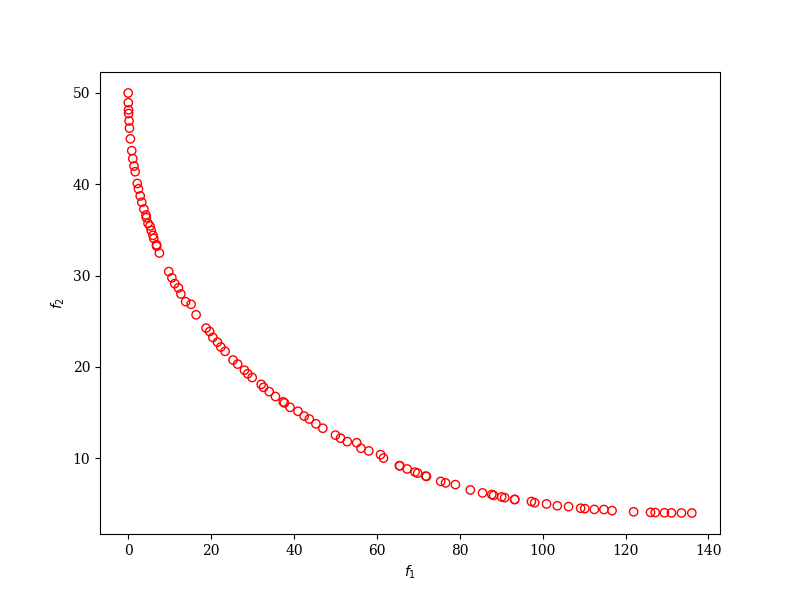
\includegraphics[width=\textwidth]{imatges/binhorn_propi.png}
        \caption{Pareto Front for Binh and Korn function}
        \label{fig:paretobinhorn}
    \end{subfigure}\hfill
    \begin{subfigure}{0.45\textwidth}
        \centering
        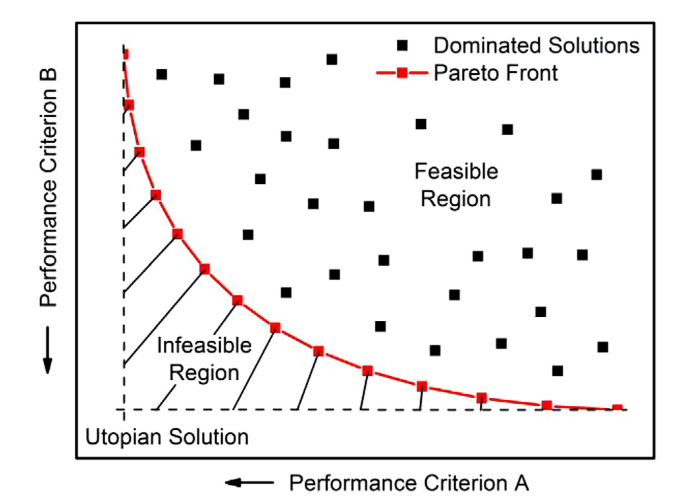
\includegraphics[width=\textwidth]{imatges/domination.png}
        \caption{Explanation of domination \cite{domination}.}
        \label{fig:domination}
    \end{subfigure}
    %\caption{Caption for both images}
    \label{fig:both_images}
\end{figure}

In Fig. \ref{fig:paretobinhorn} you can see the Pareto Front of the Binh and Korn function \cite{binhorn}, a usual test function for multi-objective optimization.

Now we can go back to our problem and decide how to define both objectives. Therefore, we define the objective function as:
\begin{equation}
    \mathbf{f}(\mathbf{x}) =(f_{invest}(\mathbf{x}),f_{tech}(\mathbf{x}))
\end{equation}
where the definition of $f_{invest}(\mathbf{x})$ is quite straight-forward; the addition of the cost of the elements in the transmission system:
\begin{equation}
    f_{invest}(\mathbf{x}) = C_{cables}(\mathbf{x}) + C_{tr}(\mathbf{x}) + C_{sh}(\mathbf{x}) + C_{gis-AC}(\mathbf{x}) + C_{ss-AC}(\mathbf{x})
\end{equation}

When it comes to how we handle  $f_{tech}(\mathbf{x})$ it becomes a little more tricky. We wanted this part to capture how optimal is the transmission system, in terms of steady-state operational conditions and power losses. In other words, this term has to measure if the inequality constraints, the ones related to operational
limits, are being satisfied and try to minimize $C_{loss_AC}$. To do so we will use a penalty method to deal with the inequality constraints.\par

Exhaustive development of this method can be found in \cite{penalty}, but the main idea is to expand the original feasible set of solutions, $ \mathbf{X}$, to all of $\mathbb{R}^n$, but a large cost or "penalty" is added to the objective function when the solution is not satisfying
 $\mathbf{G(x)} \leq 0 $. Therefore:

\begin{equation}
    f_{tech}(\mathbf{x}) = C_{loss-AC}(\mathbf{x}) + c \cdot \mathbf{p(x)}
\end{equation}

where $c$ is the penalty factor and $\mathbf{p(x)}$ is the penalty function:

\begin{equation}
    \mathbf{p(x)} = \sum_{L_i^X \in G(x)} \max(0, \mathbf{L_i(x)})
\end{equation}

In practice, setting a big value for $c$ will make the optimization method to look for solutions that satisfy the constraints.
\subsection{Algorithm Overview}

Now we have set up all the elements that define the sequential process for finding the desired Pareto Front. Now it just remains
to find the recursive optimization method that that suits best our problem. Note that here we advance that we will use the genetic algorithm
NSGA-II to solve the optimization problem (see section \ref{NSGAII}). Fig. \ref{fig:block_overview} shows the block diagram of the solver implemented in Python (check the \hyperref[Appendix]{Appendix}).

\begin{figure}[h]
\centering
\scalebox{0.95}{
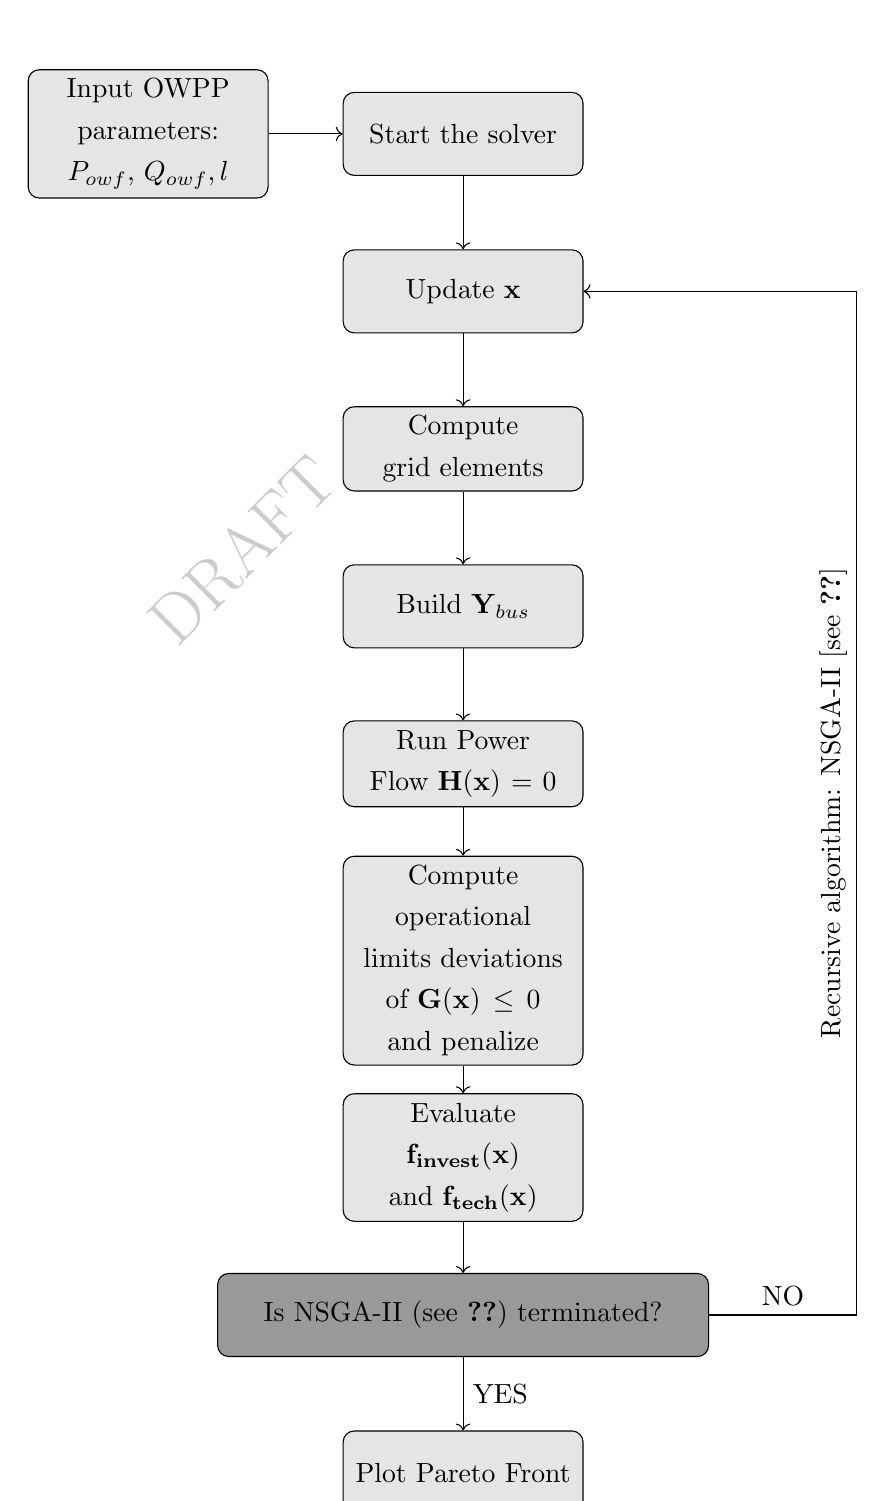
\begin{tikzpicture}[node distance=2cm, auto]
    % Define the style for the boxes
    \tikzstyle{block} = [rectangle, draw, fill=gray!20, 
                        text centered, rounded corners, minimum height=3em, text width= 8em]

    \tikzstyle{block3a} = [rectangle, draw, fill=gray!20, 
                        text centered, rounded corners, minimum height=3em, text width=6cm]

    % Define the style for the ellipses
    \tikzstyle{block?} = [rectangle, draw, fill=gray!80, 
                        text centered, rounded corners, minimum height=3em, text width=6cm]


    % Define the nodes
    \node [block] (box1) {Start the solver};
    \node [block, below of=box1] (box2) {Update $\mathbf{x}$};
    \node [block, below of=box2] (box3) {Compute grid elements};
    \node [block, below of=box3] (box4) {Build $\mathbf{Y}_{bus}$};
    \node [block, below of=box4] (box5) {Run Power Flow $\mathbf{H(x)}=0$};
    \node [block, below of=box5, yshift=-0.5cm] (box6) {Compute operational limits deviations of $\mathbf{G(x)} \leq 0$ and penalize};
    \node [block, below of=box6, yshift=-0.5cm] (box7) {Evaluate $\mathbf{f_{invest}(x)}$ and $\mathbf{f_{tech}(x)}$};
    \node [block, left of=box1, xshift=-2cm] (box3a) {Input OWPP parameters: $P_{owf}$, $Q_{owf}, l$};
    \node [block?, below of=box7] (box8) {Is NSGA-II (see \ref{NSGAII}) terminated?};
    \node [block, below of=box8] (box9) {Plot Pareto Front};
    % Connect the nodes
    \draw [->] (box1) -- (box2);
    \draw [->] (box2) -- (box3);
    \draw [->] (box3) -- (box4);
    \draw [->] (box4) -- (box5);
    \draw [->] (box5) -- (box6);
    \draw [->] (box6) -- (box7);
    \draw [->] (box3a) -- (box1); % New arrow
    \draw [->] (box7) -- (box8);
    \draw [->] (box8) -- node[midway, right] {YES} (box9);
    
    %\draw [->] (box7) to[bend right=80] node[midway,below,sloped] {Optimization method} (box2);
    \draw [->] (box8) -- ++(5,0) node[midway, above] {NO}|-  node[pos=0.25,sloped] {Recursive algorithm: NSGA-II [see \ref{fig:nsgasteps}]} (box2);
    
\end{tikzpicture}
}
\caption{Block diagram of the optimization algorithm.}
\label{fig:block_overview}
\end{figure}


\section{Optimization Methods}\label{Optimization}

After what we have summarized in the previous section we want an optimization method that:
\begin{itemize}
    \item Can handle mixed-variable optimization problems, meaning that it can handle binary, integer and continuous variables as decision vector $\mathbf{x}$.
    \item Can handle bi-objective optimization problem with equality and inequality constraints and can deal with a penalty function.
    \item Can find the whole Pareto front to analyse the trade off between the two objectives, investment and technical.
\end{itemize}

\subsection{State-of-the-art Limitations: Interior Point Method}\label{stateofart}

In \cite{paperbase} they propose an iterative method for solving the reactive power compensation problem. This methodology solves the optimization
for continuous variables using an interior point method solver \cite{ipm} for every possible combination of integer variables. Then, they compare the total
cost for all options and pick the one with smaller cost. The algorithm is summarized in Fig. \ref{fig:paaperalgo}:

\begin{figure}[H]
    \centering
    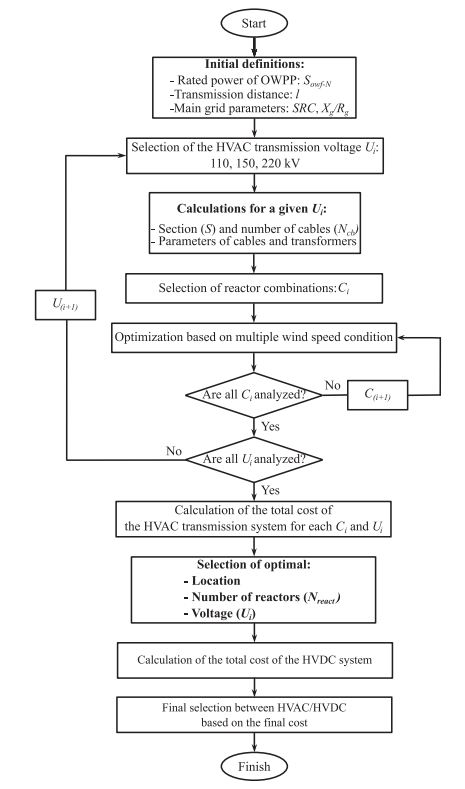
\includegraphics[width=0.4\textwidth]{imatges/paper_algo.png}
    \caption{State-of-the-art algorithm for reactive power compensation optimization \cite{paperbase}.}
    \label{fig:paaperalgo}
\end{figure}
    


This method is not suitable for our case, as we want to find the whole Pareto Front and not just one optimal solution. Moreover, the number of possible combinations of integer variables
can increase quickly in further expansions of the problem (for instance if you also consider the electrical collection system between turbines in the OWPP), making the method computationally expensive.

Another traditional method to solve multi-objective problems is to basically transform the problem into a single objective problem by using a weighted sum of the objectives \cite{nsgai}:
\begin{equation}\label{weightedsum}
    f(\mathbf{x}) = \sum_{i=1}^{k} w_i \cdot f_i(\mathbf{x}) \quad \text{where} \quad \mathbf{x} \in \mathbf{X} \text{ and } \sum_{i=1}^{k} w_i = 1
\end{equation}

From Eq. \ref{weightedsum} is clear that modifying the weights $w_i$ we change the relative importance we give to each objective. The main drawback of this approach, even though that we can deal with more than one objectives at the same time, we
still get just one solution for each combination of weights, not a set of optimal solutions, i.e. the Pareto Front. Moreover, how do we choose this $w_i$? The optimal point is sensible to these weights, therefore you must have
a clear understanding of you priorities between the objectives which is something we do not want to impose in our approach.\par

\subsection{NSGA-II: Genetic Algorithm}\label{NSGAII}



This is where genetic algorithms (GA's) come into play. GA's are a class of optimization algorithms that are inspired by the process of natural selection that uses the principles of evolution to solve optimization problems. The main idea is that they start from a random
population of candidate solutions and, in one single simulation run, they are able to find multiple Pareto optimal solutions. \par

That is why we will use the Nondominated Sorting GA II (NSGA-II) algorithm to solve our problem. It accomplishes the requirements in  section \ref{Optimization}.
Moreover, it allows us to treat inequality constraints with penalty functions, as proposed in section \ref{biobjective}.\par

An exhaustive theoretical development of how NSGA-II works is out of the scope of this work, but a complete and formal description of the algorithm can be found in \cite{NSGAII}. Just for the sake of completeness, one can simplify how NSGA-II works in the recursive steps of Fig. \ref{fig:nsgasteps}:

\begin{figure}[H]
    \centering
    \scalebox{0.95}{
    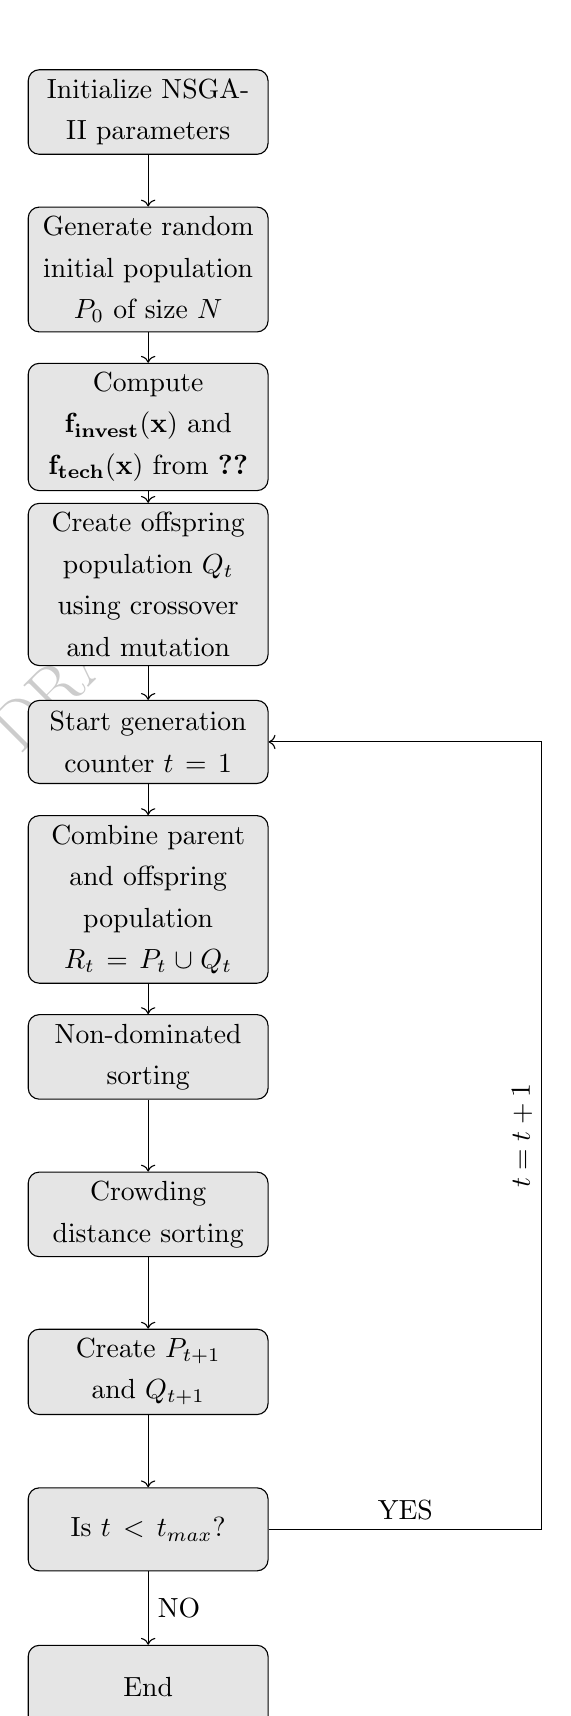
\begin{tikzpicture}[node distance=2cm, auto]
        % Define the style for the boxes
        \tikzstyle{block} = [rectangle, draw, fill=gray!20, 
                            text centered, rounded corners, minimum height=3em, text width= 8em]
    
        \tikzstyle{block3a} = [rectangle, draw, fill=gray!20, 
                            text centered, rounded corners, minimum height=3em, text width=6cm]
    
        % Define the style for the ellipses
        \tikzstyle{block?} = [rectangle, draw, fill=gray!80, 
                            text centered, rounded corners, minimum height=3em, text width=6cm]
    
    
        % Define the nodes
        \node [block] (box1) {Initialize NSGA-II parameters};
        \node [block, below of=box1] (box2) {Generate random initial population $P_0$ of size $N$};
        \node [block, below of=box2] (box3) {Compute $\mathbf{f_{invest}(x)}$ and $\mathbf{f_{tech}(x)}$ from \ref{fig:block_overview}};
        \node [block, below of=box3] (box4) {Create offspring population $Q_t$ using crossover and mutation};
        \node [block, below of=box4] (box5) {Start generation counter $t=1$};
        \node [block, below of=box5] (box6) {Combine parent and offspring population $R_t = P_t \cup Q_t$};
        \node [block, below of=box6] (box7) {Non-dominated sorting};
        \node [block, below of=box7] (box71) {Crowding distance sorting};
        \node [block, below of=box71] (box72) {Create $P_{t+1}$ and $Q_{t+1}$};
        \node [block, below of=box72] (box8) {Is $t<t_{max}$?};
        \node [block, below of=box8] (box9) {End};
        % Connect the nodes
        \draw [->] (box1) -- (box2);
        \draw [->] (box2) -- (box3);
        \draw [->] (box3) -- (box4);
        \draw [->] (box4) -- (box5);
        \draw [->] (box5) -- (box6);
        \draw [->] (box6) -- (box7);
        \draw [->] (box7) -- (box71);
        \draw [->] (box71) -- (box72);
        \draw [->] (box72) -- (box8);

        \draw [->] (box8) -- node[midway, right] {NO} (box9);
        
        %\draw [->] (box7) to[bend right=80] node[midway,below,sloped] {Optimization method} (box2);
        \draw [->] (box8) -- ++(5,0) node[midway, above] {YES}|-  node[pos=0.25,sloped] {$t=t+1$} (box5);
        
    \end{tikzpicture}
    }
    \caption{Block diagram of NSGA-II}
    \label{fig:nsgasteps}
    \end{figure}

Regarding the description of the algorithm in Fig. \ref{fig:nsgasteps}:
\begin{enumerate}
    \item Initially a random population $P_0$ of size $N$ is created. This population is sorted according to non-domination (which is an equivalent name for Pareto dominance) described in  Eq. \ref{paretodomination}.
    \item A new offspring population $Q_t$ is created by applying crossover and mutation operators to the population $P_t$. Crossover combines two solutions $\mathbf{x}$'s to create a new one and mutations introduce small random changes, or mutations, to $\mathbf{x}$.
    This part is where the inspiration for the name of GA's comes from. Check \cite{NSGAII} for further explanation.
    \item The offspring population $Q_t$ is combined with the parent population $P_t$ to create a new population $R_t$ of size $2N$. This population is sorted again according to non-domination.
    \item Non-dominated sorting creates non-dominated sets $F_i$ of solutions where $i$ is the non domination level.
    The first set $F_1$ contains the non-dominated solutions, the second set $F_2$ contains the solutions that are dominated only by the solutions in $F_1$ and so on.
    \item Crowding distance sorting basically creates the new $P_{t+1}$ by selecting the best solutions in the non-dominated sets $F_i$ until you arrive to size of $N$ for the new population.
    \item The algorithm iterates until the maximum number of generations $t_{max}$ is reached, which will be the termination condition.

\end{enumerate}

\begin{figure}[H]
    \centering
    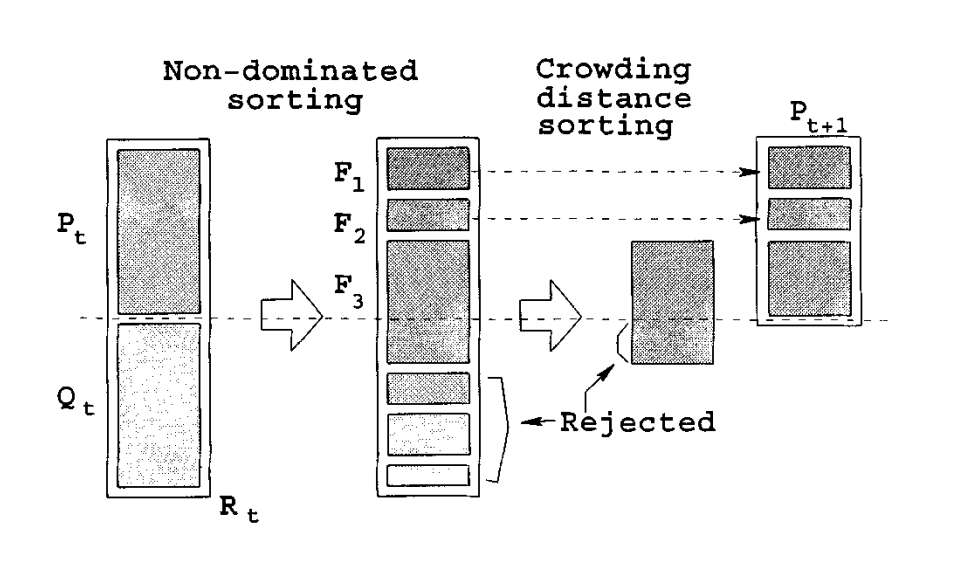
\includegraphics[width=0.5\textwidth]{imatges/proces_nsga.png}
    \caption{Visualization of steps 4 and 5 \cite{NSGAII}.}
    \label{fig:stpesnsga}
\end{figure}

The algorithm in Fig. \ref{fig:block_overview} has been implemented in pymoo \cite{pymoo}, a Python library for multi-objective optimization that includes the NSGA-II algorithm \ref{fig:nsgasteps} and allows formulating mixed-variable problems.
It is worth mentioning that the proposed method in Fig. \ref{fig:block_overview} is performed on a whole set of $N$ candidate solutions $\mathbf{x}$ from the population set $P$.




\subsection{Optimal Power Flow Approach for Compensation Optimal Sizing}

In this section we propose a different approach based on the Optimal Power Flow (OPF) to validate the results obtained with NSGA-II, specifically the ones relates to
the sizing of the reactive power compensation.\par 

The idea is to take one optimal solution from NSGA-II, i.e. all the decision variables in $\mathbf{x}$, and recompute just the values of sizing of the shunt reactors $Y_{sh_i}$. The main idea is to compare how close is the 
stochastic approach solutions of NSGA-II to the solutions given by a standard deterministic approach as the OPF. \par


The traditional AC-OPF objective function \cite{opfnotes} minimizes de cost of generating active power:
\begin{equation}
    \underset{P_G}{\text{min}} \quad \mathbf{c^T} \mathbf{P_G} \quad \text{where} \quad \mathbf{c} = \begin{bmatrix} c_0 \\ c_1 \\ c_2 \end{bmatrix}
\end{equation}
where $\mathbf{P_G}$ is the vector of active power generated by the generators and $c_0$, $c_1$ and $c_2$ are the independent, linear and quadratic power generations costs respectively.

As we saw in Eq. \ref{eq:shuntcost}, shunt reactors compensate a reactive power equivalent to $Q_{sh} = Y_{sh} \cdot U^2$. Therefore, finding the optimal size of the shunt reactors is equivalent
to minimize the cost of the reactive power compensation. Therefore,  we can modify the objective function of the OPF to:

\begin{equation}\label{eq:Qopf}
\underset{Q_{sh}}{\text{min}} \quad \mathbf{c_{sh}^T} \mathbf{Q_{sh}} \quad \text{where} \quad \mathbf{c_{sh}} = \begin{bmatrix} K \\ P \\ 0 \end{bmatrix}
\end{equation}
where K and P are from Table \ref{tab:parametersshunt}.\par
We have made this modifications implemented in the AC-OPF solver in GridCal \cite{gridcal}, an open-source Python library for power systems analysis. Note that the derivatives of the objective functions, Jacobian and Hessian, have
been modified according to the new objective function \ref{eq:Qopf}.


\section{Case Study}\label{CaseStudies}

In this section we will study in depth the results that the algorithm yields for a specific design parameters
of an OWPP. We will benchmark the results obtained with NSGA-II with a "brute" force approach using random search and compare the results of reactors sizing comparing with the OPF
approach. Moreover, we will do an in-depth analysis of the optimal solution cost breakdown and compare it to optimal points without considering reactive power compensation to understand the need
to include this in the optimization problem.



The results obtained have been computed in a laptop with the following specifications:
\begin{itemize}
    \item Processor: Processor: Intel(R) Core(TM) i5-8365U CPU @ 1.60GHz
    \item RAM: 8 GB
    \item OS: Windows 11
    \item IDE: Visual Studio Code and PyCharm
    \item Python version: 3.11.8
    \item Pymoo version: 0.6.1
    \item GridCal version: 5.1.11
\end{itemize}

The tuning parameters used for initializing the NSGA-II algorithm are shown in Table \ref{tab:NSGAII_parameters}.

\begin{table}[h]
\centering
    \begin{tabular}{l|l}
    \hline
    \textbf{Parameter} & \textbf{Value} \\ \hline
    Population size, $N$ & 150 \\ \hline
    Survival sorting & Rank and Crowding $"pcd"$ \\ \hline
    Termination, $t_{max}$  & 15 generations \\ \hline
    constraint penalty, $c$ & 10e4 \\ \hline
    \end{tabular}
    \caption{Tuning parameters NSGA-II.}
    \label{tab:NSGAII_parameters}
\end{table}

It is worth mentioning that NSGA-II has a time complexity of $\mathcal{O}(MN^2)$, where $M$ is the number of objectives and $N$ the population size. With $M=2$ and setting $N=150$ and $t_{max}=15$,
it takes the algorithm about $10$ s to terminate. To put this performance in perspective, the method proposed in \cite{paperbase} and described in section \ref{stateofart} needs between $45$ and $140$ s to find the optimal solution.


\subsection{500 MW, 100 km OWPP}

We pick as case study a 500 MW OWPP located 100 km from shore. Results have been separated in different subsections to study specific results.

\subsubsection{Random Search compared to NSGA-II}

In this section we compare the results obtained with NSGA-II with a brute force approach. This simply means that we generate a random population of solutions within certain bounds that guarantee power flow convergence on most of the cases and evaluate the objective function with those solutions.
For the sake of a fair comparison, we showcase the results obtained with the two methods at the same computation time of around $10$ s, which corresponds to 700 random evaluations.

In Fig. \ref{fig:searchall} we can see how both the NSGA-II and the random search are distributed in the objective function $\mathbf{f(x)}$ 2-D space. To give some intuition on what we see, each set of black points (random evaluations) is characterized by a dominant term in the investment cost value, normally the number of cables or the placing 
of a shunt reactor mid-cable both of which introduce big changes in the investment cost. The red points (NSGA-II) is the set of Pareto dominating solutions.
\begin{figure}[H]
    \centering
    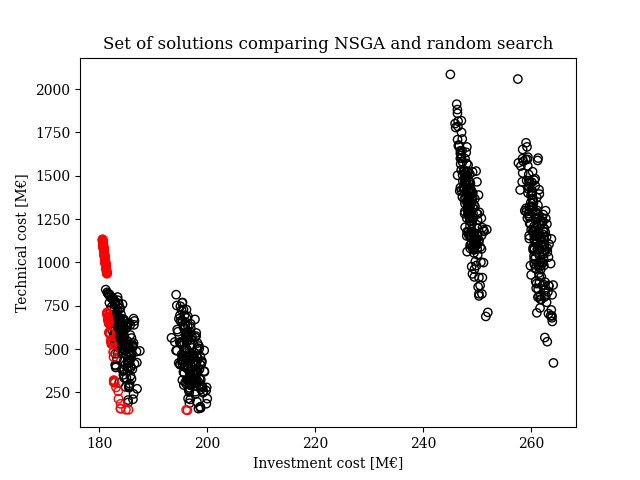
\includegraphics[width=0.7\textwidth]{imatges/random_vs_nsga_all.png}
    \caption{Random search (black) compared to NSGA-II (red).}
    \label{fig:searchall}
\end{figure}

From the results in Fig. \ref{fig:searchall} and the zoom on the Pareto area on Fig. \ref{fig:paretpnsga} we can see that:
\begin{itemize}
    \item NSGA-II is able to find the set of optimal solutions in the region closer to the utopia point, i.e. where both objectives are equal to 0.
    \item The Pareto front is well-defined and the solutions are well distributed.
    \item NSGA-II is able to find solutions that are non-dominated by the random search. This means that the algorithm effectively outperforms any kind of brute force approach
    since it reveals a  set of solutions $F_1$ that dominates all the random search points.
\end{itemize}


\begin{figure}[H]
    \centering
    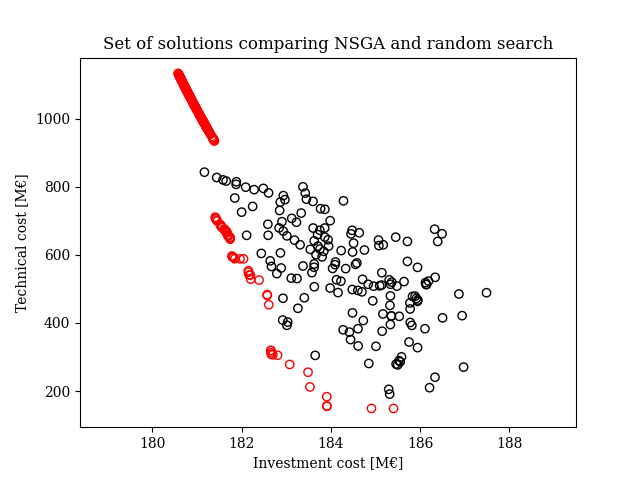
\includegraphics[width=0.7\textwidth]{imatges/random_vs_nsga_zoom.png}
    \caption{Zoom on the Pareto Front area, random search (black) compared to NSGA-II (red).}
    \label{fig:paretpnsga}
\end{figure}

Note in Fig. \ref{fig:paretpnsga} we see a weird behaviour on the upper-left side of the Pareto front. It seems that in that region, the one corresponding to not including any shunt reactor, there are some random search points that dominate the NSGA-II
results. This should not be the case and our hypothesis is that it is related to the random sampling of binary variables (the one corresponding to the locations of the shunt reactors) of the initial population $P_0$ and how is unable to generate a well-distributed population of candidate solutions.
Future work should focus on how to improve the initial population sampling of all types of variables and hopefully solve this issue. 


\subsubsection{OPF Validation}

Now we showcase how the OPF approach helps to validate the results obtained with NSGA-II. We pick one point from the Pareto Set and  take its solution for all the variables in $\mathbf{x}$
except for the continuous variables of the sizing of the reactors, $Y_{sh_i}$.

We will use a random point of the non-dominated set, arbitrarily chosen to be the one minimizing both objectives with equal weights. This essentially is converting the multi-objective problem into a single objective one using the method proposed in section \ref{stateofart} with $w_{invest} = w_{tech} = 0.5$. The optimal solution we get from NSGA-II is
presented in Table \ref{table:optimalvaluesdicrete}:

\begin{table}[H]
    \centering
    \begin{tabular}{l l}
    \hline
    \textbf{Parameter} & \textbf{Value} \\
    \hline
    Transmission voltage level & 220 kV \\
    Number of cables & 2 \\
    Reactors & $[1, 1, 0, 1, 0]$ \\
    Rated power of the transformer & 509.72 MVA \\
    \hline
    \end{tabular}
    \caption{Specifications (excluding reactors sizing) of the optimal solution.}
    \label{table:optimalvaluesdicrete}
    \end{table}

Now, we run the OPF proposed in Eq. \ref{eq:Qopf} and implemented in GridCal and compare the results. Initially, we check the convergence and running time of the OPF:
\begin{figure}[H]
    \centering
    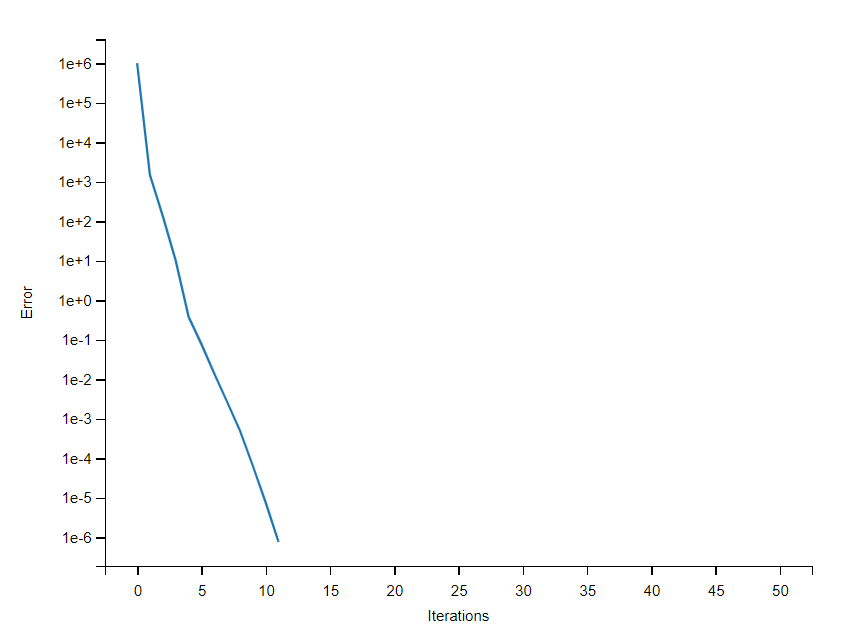
\includegraphics[width=0.75\textwidth]{imatges/opf_convergence.png}
    \caption{OPF convergence}
    \label{fig:opfconv}   
\end{figure}

Fig. \ref{fig:opfconv} shows how the OPF converges to the optimal solution in 12 iterations, and it takes about 1.5 seconds. For comparison, running the traditional PF in \ref{NRsolver} takes around 0.06 s.
That makes OPF around 25 times slower than the traditional PF.



Afterwards, we check the values $Y_{sh}$ obtained from the OPF and see how they affect the objective function:
\begin{figure}[H]
    \centering
    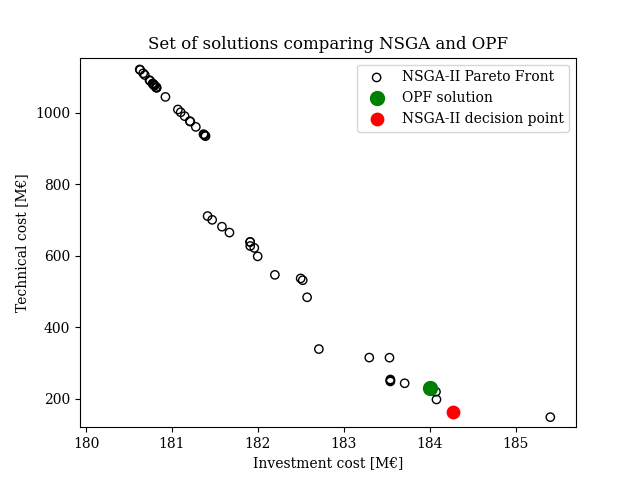
\includegraphics[width=0.75\textwidth]{imatges/opf_vs_nsga.png}
    \caption{NSGA-II vs OPF for reactors sizing.}
    \label{fig:opfvsnsga}   
\end{figure}

As we see in Fig. \ref{fig:opfvsnsga}, the OPF gives a solution that is very close to the one obtained with NSGA-II and most importantly, the OPF solution does not dominate the NSGA-II solution. The fact that the point is not exactly the same is because OPF and NSGA-II penalization costs are defined differently and
cannot be compared directly. Nevertheless, the important property is that both solutions fall in the same Pareto front.

This validates the results obtained with NSGA-II since OPF, which is a strictly traditional optimization method, does fall on the same non-dominated set $F_1$, meaning that it has not found a combination of reactors sizing that Pareto 
dominates the solutions from NSGA-II.

\subsubsection{Costs Break Down}

In this section we will break down the investment costs terms of the optimal solution presented in Table \ref{table:optimalvaluesdicrete} and compare it to the same solution eliminating the reactive power compensation given by the shunt reactors. The idea is to quantify to effect of reactive power compensation
in the power losses of the transmission system and the need to include it in the optimization problem. The results are presented in Fig. \ref{fig:nsgacosts} and Fig. \ref{fig:noshcosts}:

\begin{figure}[H]
    \centering
    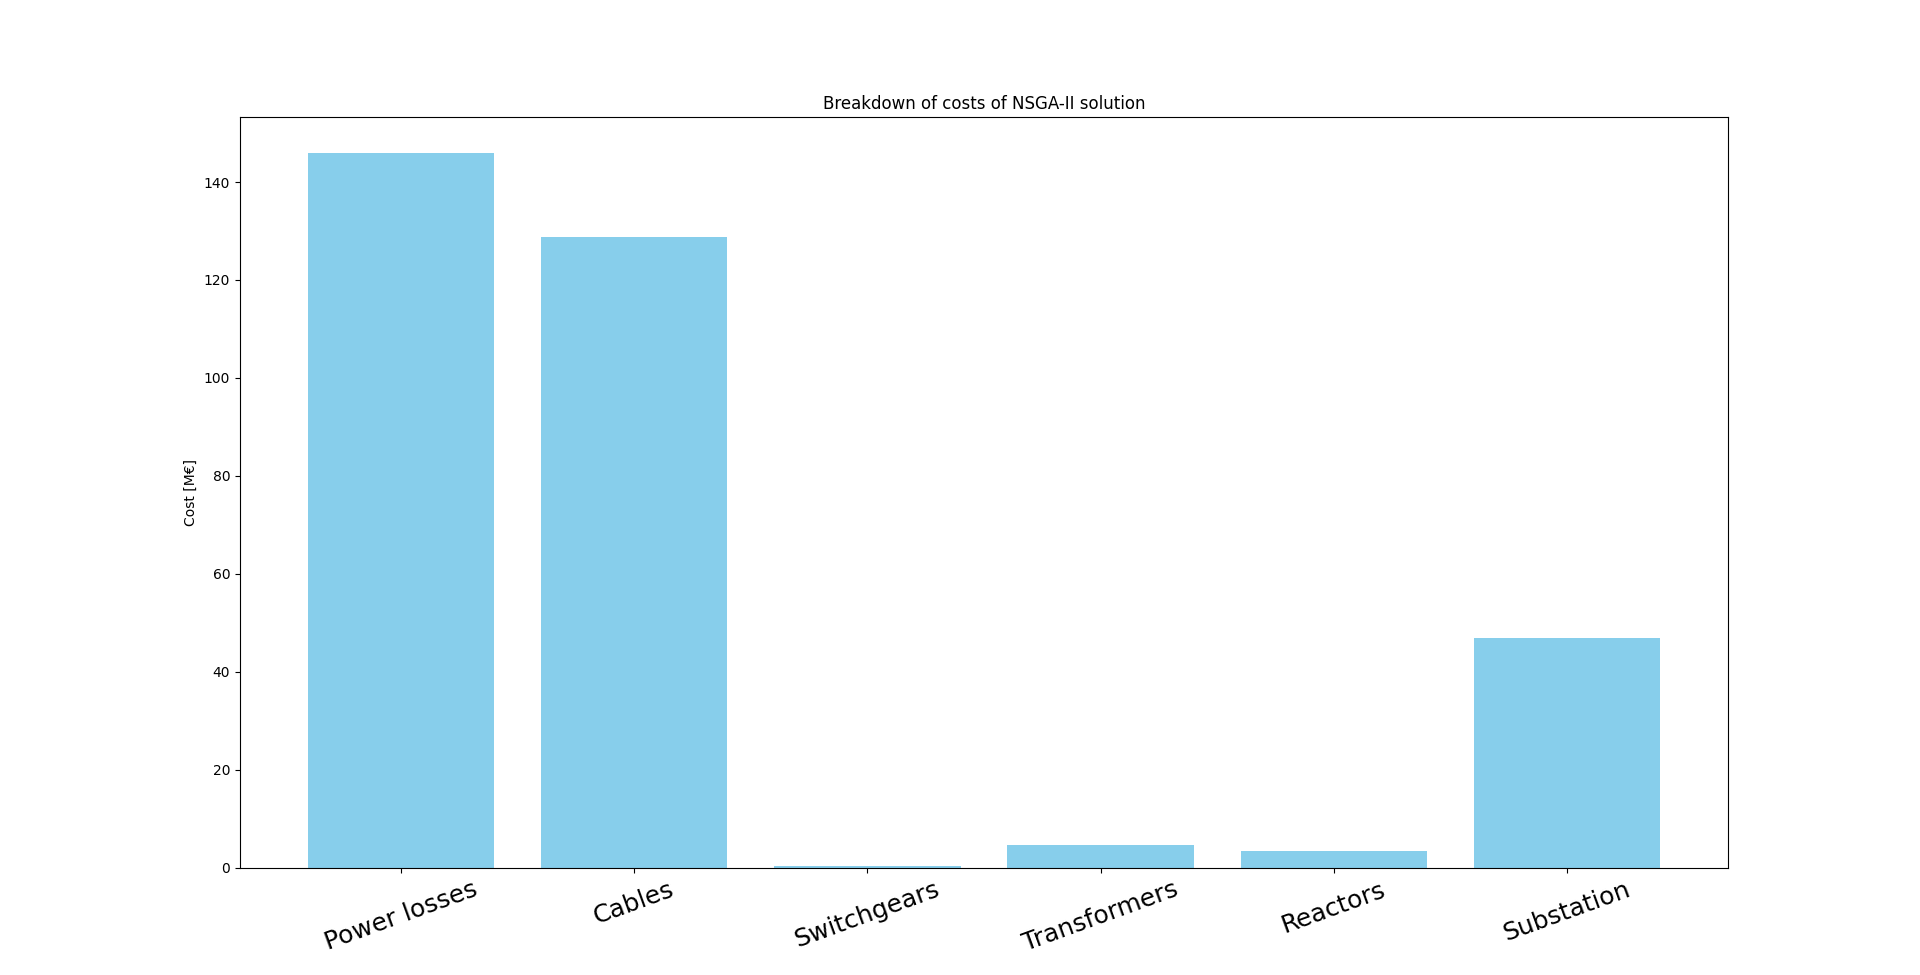
\includegraphics[width=1.0\textwidth]{imatges/cost_nsga.png}
    \caption{NSGA-II optimal solution cost break down.}
    \label{fig:nsgacosts}
\end{figure}

\begin{figure}[H]
    \centering
    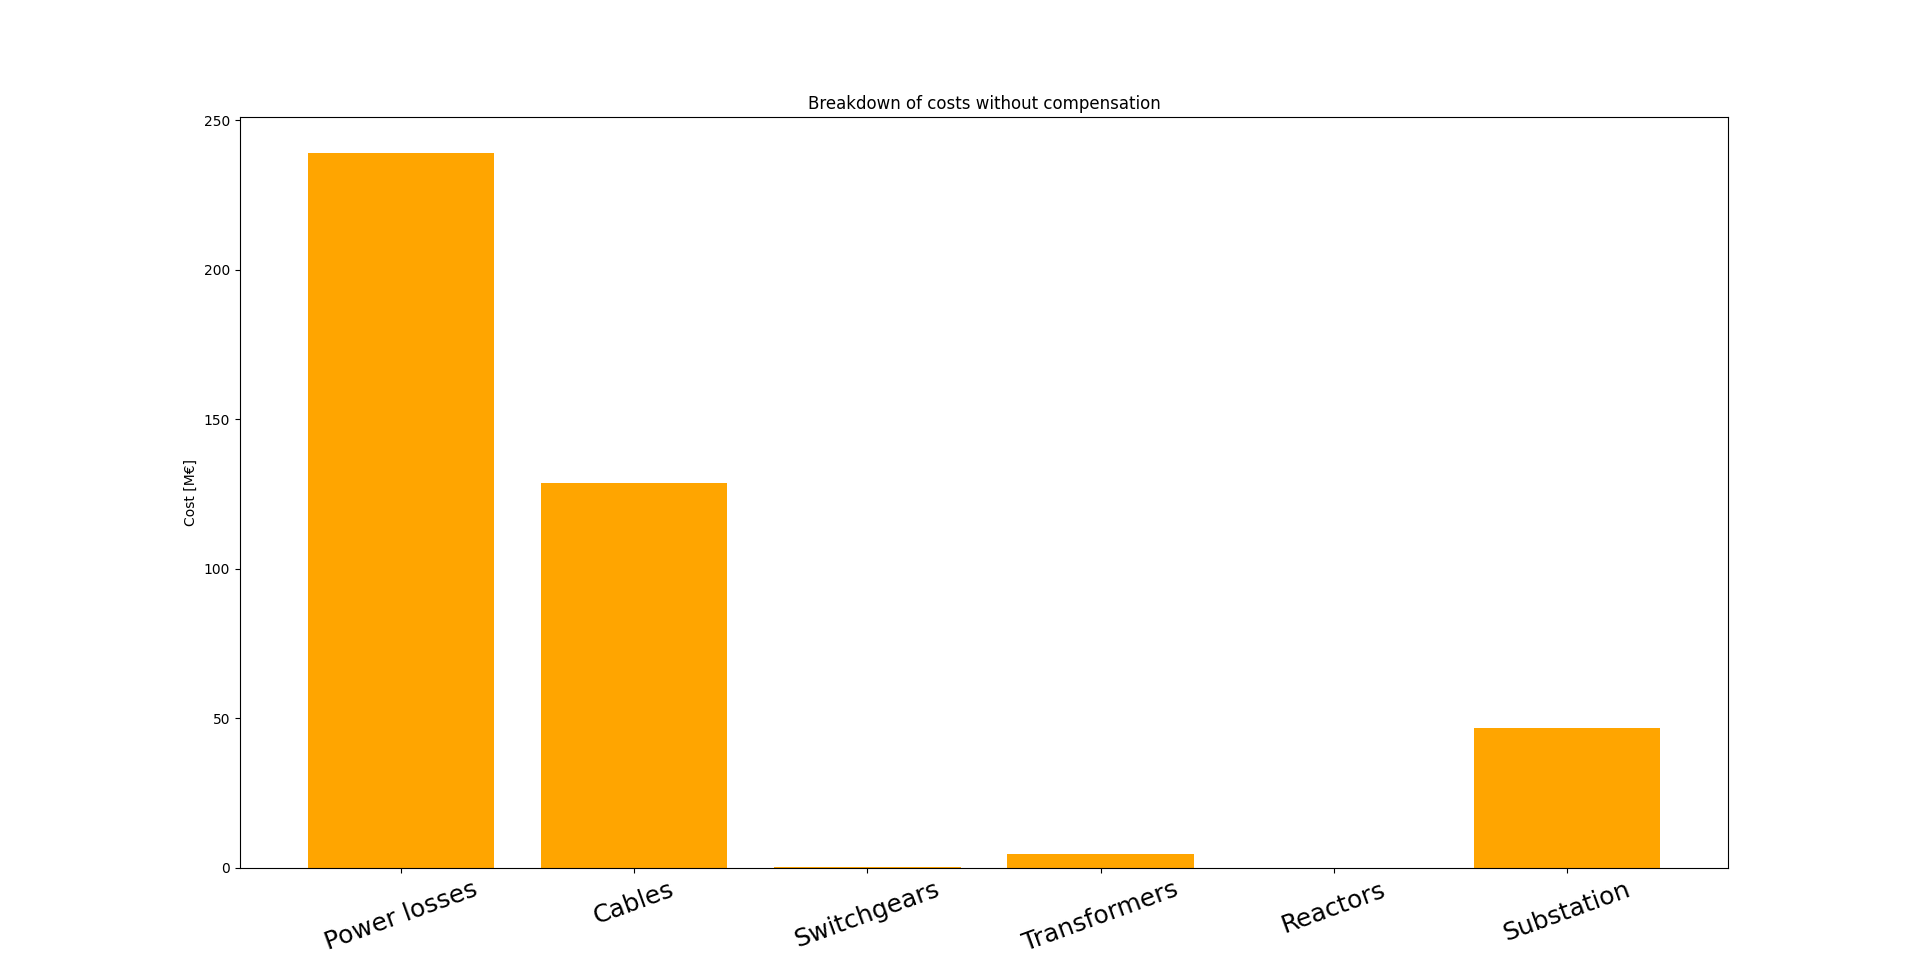
\includegraphics[width=1.0\textwidth]{imatges/costs_nosh.png}
    \caption{No compensation solution cost break down.}
    \label{fig:noshcosts}
\end{figure}
Note the different scales in the y-axis of Fig. \ref{fig:nsgacosts} and Fig. \ref{fig:noshcosts} and how power losses, cables and substation cost are the dominant ones. For the sake of clarity 
we can compare both cumulative total costs in the same plot as seen in Fig. \ref{fig:coparativecosts}:
\begin{figure}[H]
    \centering
    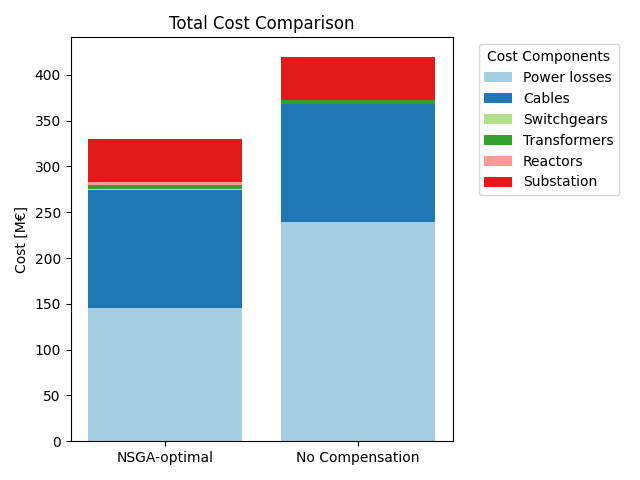
\includegraphics[width=0.7\textwidth]{imatges/cost_comparision.png}
    \caption{NSGA-II optimal solution and no-compensation total cost comparison.}
    \label{fig:coparativecosts}
\end{figure}

The main conclusions we can extract from the results in Fig. \ref{fig:coparativecosts} is that the cost of including shunt reactors is very profitable since an extra
$ 3.35 M\euro$ in investment cost is translated into a $ 93.2 M\euro$ reduction in the power losses costs, an impressive $ 39 \% $ reduction.

From this section the need of reactive power compensation is clear. Moreover, future work presented in the next section \ref{injectionevol} and in section \ref{futurework} will showcase how this compensation becomes even more important when we consider 
a variable power injection from the OWPP.

\subsubsection{Power Losses and Overvoltage with Variable Power Injection} \label{injectionevol}

This section will serve as a breeding ground for future work, check \ref{futurework}. We want to see how the power losses and overvoltages evolve with power injections below the nominal value using the optimal solution we have found considering that $P_{owf} = 500$ MW always. Also, we will check what happens if we eliminate the reactive power compensation to 
compare how effective is to include these shunt reactors in the optimization problem.  The results are presented in
Fig. \ref{fig:lossesevol} and Fig. \ref{fig:overvoltevol}:

\begin{figure}[H]
    \centering
    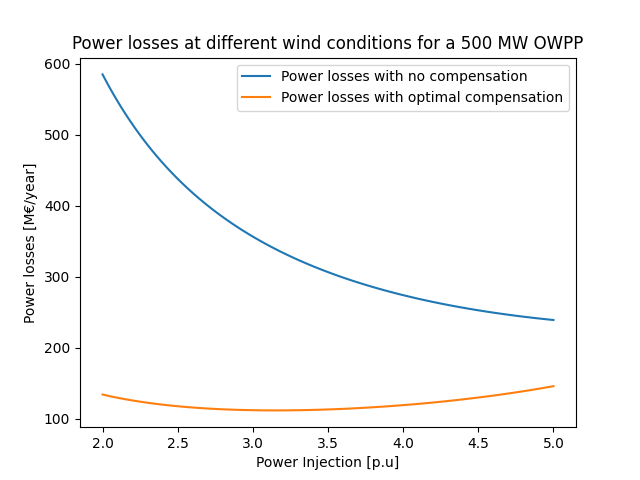
\includegraphics[width=0.7\textwidth]{imatges/losses evolution.png}
    \caption{Power losses evolution with variable power injection.}
    \label{fig:lossesevol}
\end{figure}

From Fig. \ref{fig:lossesevol} we see how the power losses increase exponentially as we reduce $P_{owf}$ when no reactive power
compensation is considered. This is due to the fact that the power losses are directly proportional to the square of the current in the transmission lines and the reactive power compensation helps to reduce it when $p_{owf}$ decreases.
As to the optimal compensation solution we observe that power losses (as expected from \ref{fig:whycomp}) are kept relatively low for all power injections considered, showcasing how useful shunt reactors are for limiting power losses in presence of variability of
the power injection.
\begin{figure}[H]
    \centering
    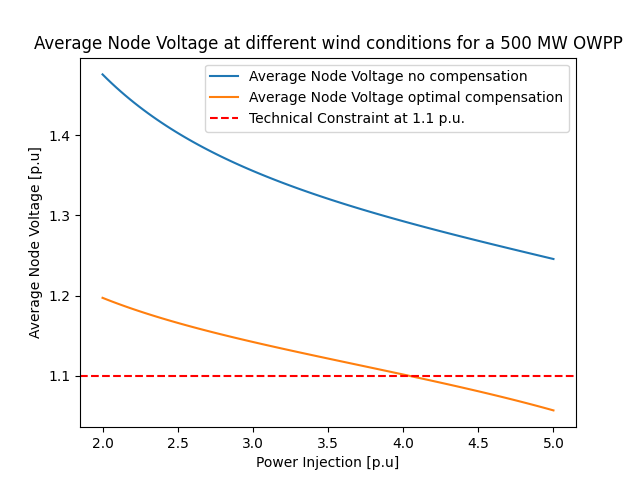
\includegraphics[width=0.7\textwidth]{imatges/overvoltageplot.png}
    \caption{Overvoltage evolution with variable power injection.}
    \label{fig:overvoltevol}
\end{figure}

From Fig. \ref{fig:overvoltevol} we see that reducing the power injection also increases $V_{avg}$, which is the average of all nodes in the transmission system voltage level in p.u. Again, shunt reactors effectively manage to keep $V_{avg}$ below the limit of $1.1$ p.u. (which no compensation cannot do) but up to a certain point where the power injection is so low that the shunt reactors are not able to compensate the reactive power enough to keep the voltage level below the technical limit. It
is clear from the optimization in Eq. \ref{optiprob} that if we want to satisfy operational limits, we need to increase the reactive power compensation in the optimal solution if lower $P_{owf}$ are considered.

Considering a distribution for the wind speed, as proposed in section \ref{futurework}, will include this distribution of power injections below the nominal value and will give a more realistic view of the system and the need for reactive power compensation.


%------------------------------------------
\section{Conclusions}\label{Conclusions}

All the objectives proposed at the beginning in section \ref{objectives} have been accomplished. This chapter summarizes
the main conclusions of the work and presents some proposals to take into consideration for future
related work.

\subsection{Outcome}

The main outcomes derived from the objectives met from each chapter of interest are:
\begin{itemize}
    \item Chapter \ref{Minimization} covers the  mathematical fundamentals of the problem formulation and optimization approach. The analysis shows how the multi-objective approach helps us achieve
    the desire to obtain the full Pareto Front and how this approximation becomes useful to understand the underlying behaviour of the power flow analysis of the transmission system model.

    \item Chapter \ref{Optimization} presents the state-of-the-art optimization algorithm and presents the different techniques that have been considered to be used.
    It establishes the limitations that have been found and how the applications of a genetic algorithm such as NSGA-II
    can help to overcome them and meet the requirements of the optimization problem. It presents some theoretical fundamentals of the algorithm used and the schematic of the recursive solver that has been implemented.

    \item Chapter \ref{CaseStudies} applies the optimization algorithm to a specific case study of an OWPP. First, the algorithm implementation has been demonstrated to be fully functional and meets the requirements in section \ref{Optimization}.
    The results show how we obtain a coherent Pareto Front and how the results obtained outperform any brute force approach, revealing a set on non-dominated optimal solutions. Moreover, the comparison with the OPF approach validates our results and shows that
    NSGA-II is able to reach the "best" points using a stochastic approach given that OPF is unable to explore any dominating area below the Pareto Front. The cost breakdown and evolution of cots for different power injections give an intuitive 
    explanation of the need for reactive power compensation.\par
    All in all, it can be concluded that the innovative approach of using a GA for the optimization of the transmission system of an OWPP has been successful, and it has promising properties as a potential powerful tool to deal with this kind of optimization
    with reduced computational time.

\end{itemize}

\subsection{Future Work}\label{futurework}

The implementation of NSGA-II for the optimization of OWPP transmission system design has potential to become a powerful tool. In this section we will propose a set of possible improvements
that could enhance the overall quality of the proposed method and give new insights.\par 

The main simplification and assumption through the development of the work has been assuming a constant power supplied by the OWPP
at its nominal value, in other words, we are assuming a constant wind speed at the desired value. As shown in Fig. \ref{fig:whycomp} and in section \ref{injectionevol}, the need of reactive power compensation increases as the power injections of our plant decreases, i.e. low wind or no wind.
The next and logical step is to let the proposed algorithm to consider different wind conditions. To be more accurate, we should consider a wind speed distribution, normally assumed to follow a Weibull distribution shown in Fig. \ref{fig:weibull}.

\begin{figure}[H]
    \centering
    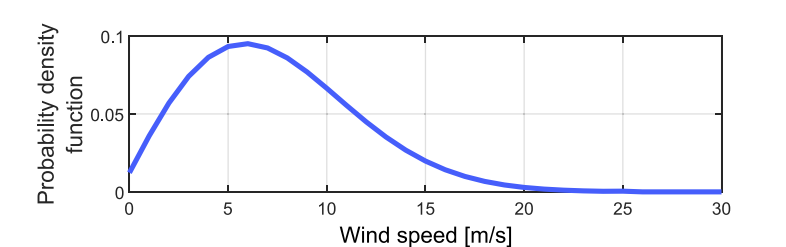
\includegraphics[width=0.7\textwidth]{imatges/weibull.png}
    \caption{Weibull's distribution of wind speeds \cite{paperbase}.}
    \label{fig:weibull}
\end{figure}

To consider this distribution, we propose to create a set of N wind speeds $u_j$,  and associate a probability $p_j$ and power generation $P_{owf_j}$ to each of them. Now it would just remain that the step on which we solve the power flow in Fig. \ref{fig:block_overview} to compute a 
weighted average of the power injections of the OWPP, $P_{owf}$  with the probabilities $p_j$. Doing so, the objective function will be a weighted sum of the costs of the different wind conditions:
\begin{equation}
\begin{aligned}
        f_{invest}(\mathbf{x}) &= \sum_{j=1}^{N} p_j \cdot  \left[ C_{cables}(\mathbf{x}) + C_{tr}(\mathbf{x}) + C_{sh}(\mathbf{x}) + C_{gis-AC}(\mathbf{x}) + C_{ss-AC}(\mathbf{x}) \right] \\
        f_{tech}(\mathbf{x}) &= \sum_{j=1}^{N} p_j \left[ \cdot C_{loss-AC}(\mathbf{x}) + c \cdot \mathbf{p(x)} \right] \\       
\end{aligned}   
\end{equation}

This approach will give a more realistic view of the system and allow to do a fair comparison between the state-of-the-art results in terms of reactive power compensation sizing for every different combination of $P_owf$ and $l$ for OWPP. \par

Moreover, recall that we have limited our work to the HVAC technology, but HVDC technology should also be considered as an option.
Literature \cite{paperbase} shows that after considering shunt reactors for reactive power compensation purposes, after the break-even distance of around 150 km,
using HVDC becomes cheaper than HVAC, for which power losses increase notably for high distances. Computing costs for HVDC would allow to extend the decision variables of the optimization to its full
domain of possibilities.\par

Moreover, further work could be to consider how disturbances of the voltage of the grid we are supplying to or the layout of the electrical collection system (see Fig. \ref{layouts_shape}) inside the OWPP could affect the optimization problem. 
Also, this work could be implemented in a software like GridCal. Implementing this algorithm in an open-source software would allow to make it accessible to a wider audience, with a more user oriented interface and to be used in real-life projects.

\begin{figure}[H]
    \centering
    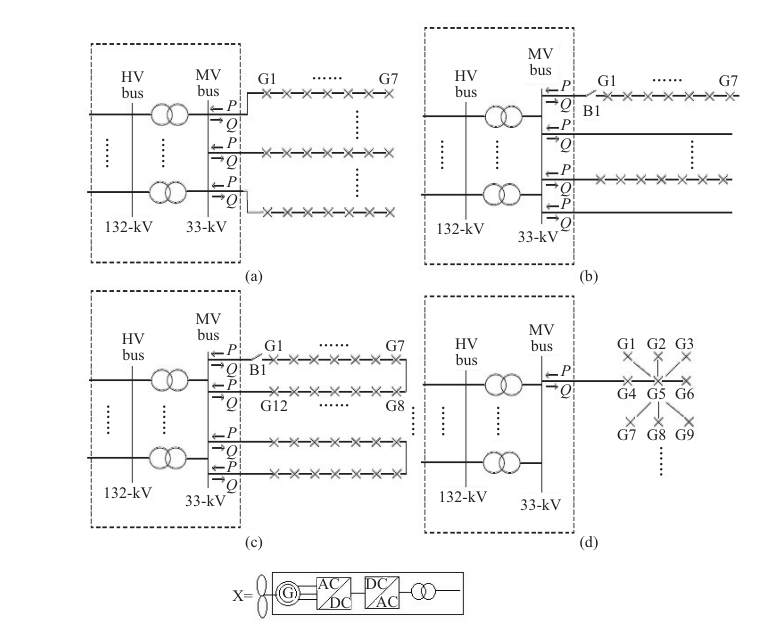
\includegraphics[width=0.5\textwidth]{imatges/layouts.png}
    \caption{Collection system for some OWPP possible layouts: Radial(a), Single-sided ring(b), Double sided ring(c) and star(d) \cite{layouts_coll}.}
    \label{layouts_shape}
\end{figure}

Finally, one of the main criticism to this work would be the validity of the cost functions used for the objective function. Finding and approximating this functions is no easy work,
since costs associated to each element vary from manufacturer to manufacturer and cost analysis can be extended not just initial investment ones, but to other concepts such as maintenance, operation and depreciation costs. Studying more complex and accurate 
versions of costs functions is another potential line of work.\par

All in all, the work developed in this thesis provides a good theoretical and practical basis for further research in the optimization of transmission systems in OWPP. In fact, this thesis will be used as the starting point for eRoots and Acciona to implement an operative and complete version of the algorithm in GridCal.
%------------------------------------------
\section{Planning and Viability Studies}\label{Planning}

\subsection{Time Planning}

Fig. \ref{fig:gantt} shows the time distribution for the tasks carried out in the thesis.
\begin{figure}[h]
\begin{center}
\begin{ganttchart}[hgrid, vgrid]{1}{20}
    \gantttitle{Thesis Gantt Chart}{20} \\
    \gantttitle{February}{4} \gantttitle{March}{4} \gantttitle{April}{4} \gantttitle{May}{4} \gantttitle{June}{4} \\
    \ganttbar{Literature review}{1}{6} \\
    %\ganttlinkedbar{Task 2}{2}{3} \ganttnewline
    \ganttbar{Modelling of the grid}{3}{7} \\
    \ganttbar{Power flow solver}{6}{8} \\
    \ganttlinkedbar{Optimization methods}{9}{18} \\
    %\ganttbar{Optimization methods}{9}{18} \\
    \ganttbar{Case study}{12}{18} \\
    \ganttbar{Thesis final writing}{17}{20}
    \ganttlink{elem0}{elem3}
    \ganttlink{elem3}{elem4}
    \ganttlink{elem1}{elem2}
\end{ganttchart}
\caption{Thesis Gantt Chart.}
\label{fig:gantt}
\end{center}
\end{figure}

\subsection{Economic Assessment}

The budgeting for this work includes the human resources used during the development of the thesis. We have considered the working hours devoted to the project under the internship agreement, as well as an average of 2.5 hours per week of tutor supervision.
The total cost has been broken down with and without the Value Added Tax (VAT). The complete budgeting is shown in Table \ref{tab:costs}.
\begin{table}[h]
\centering
\begin{tabular}{c c c c}
\hline
\textbf{Concept} & \textbf{ Unit Cost} & \textbf{Quantity} & \textbf{ Total (\euro)} \\
\hline
Working hours & 8 \euro/h  & 450 h & 3600 \\
Tutor supervision & 25 \euro/h   &  50 h & 1250 \\
\hline
\textbf{Total without VAT} & & & 4850 \\
\hline
\textbf{Total with VAT (21\%)} & & &  5868.5 \\
\hline
\end{tabular}
\caption{Thesis Costs.}
\label{tab:costs}
\end{table}

Note that the computer used for the development of the thesis has not been included in the budgeting, as it was already owned by the author and well-beyond its amortization period.

\subsection{Environmental Assessment}

\subsubsection{Energy Consumption}

This environmental assessment evaluates the energy consumption costs incurred during
the development of a thesis over five months, using a computer as the primary tool. The primary energy consumption arises
from the computer's usage, which includes writing, research, data analysis, and communication.\par

Assuming an average laptop with a power consumption of 60 watts, used for approximately 6 hours daily, the total energy consumption
over five months is around 54 kWh. This consumption translates to roughly 30 kg of CO2 emissions, assuming the average emission
factor for electricity generation.\par

To reduce these energy costs and associated environmental impacts in future thesis projects, several strategies can be employed.
Utilizing energy-efficient computers, enabling power-saving modes, and limiting usage time can significantly lower consumption.
Additionally, adopting renewable energy sources, such as solar panels for charging devices, further reduces the carbon footprint,
contributing to a more sustainable academic practice.

\subsubsection{Potential Impact}

Optimizing transmission systems in OWPP can significantly enhance environmental impact by maximizing energy efficiency
and reducing carbon emissions. Improved transmission reduces energy losses, ensuring that more clean energy reaches the grid, thereby displacing fossil
fuel-based power generation. Additionally, optimization can lead to less intrusive infrastructure, minimizing harm to marine ecosystems and reducing the physical footprint of OWPP.
Efficient transmission systems also facilitate the integration of larger amounts of renewable energy, supporting the transition to a sustainable energy future and helping to combat climate change by lowering
greenhouse gas emissions.









\subsection{Social and Gender Equality Assessment}

This assessment evaluates the social and gender equality aspects of a bachelor's thesis focused on developing a tool for optimizing renewable energy system design, authored by a 22-year-old white engineering student. While the thesis itself addresses a critical area in sustainable development, examining its social dimensions is essential to ensure inclusivity and equality.

The demographic profile of the author reflects broader trends in STEM fields, where women and minority groups remain underrepresented. This lack of diversity can influence the perspectives and priorities embedded in the research. Ensuring diverse representation in such projects is crucial for incorporating a wide range of insights and addressing the needs of various communities.

To promote social and gender equality, the research should consider the differential impacts of renewable energy systems on diverse populations. This approach ensures that the developed tools and technologies are accessible and beneficial to all segments of society.

Moreover, educational institutions should encourage and support participation from diverse backgrounds in engineering and renewable energy fields. Mentorship programs, scholarships, and targeted recruitment can help bridge the gender and social gap, fostering an environment where innovative solutions for renewable energy are developed through diverse and inclusive contributions.
%------------------------------------------


\section*{Acknowledgements}
 \addcontentsline{toc}{section}{Acknowledgements}

Primer de tot vull agraïr profundament el suport constant del Josep, el meu tutor, que m'ha donat consell i ajuda quan
l'he necessitada cada dia des de que vaig entrar a eRoots. Per extensió, agraïr la rebuda i suport de tot l'equip d'eRoots durant aquests mesos,
especialment al meu tutor acadèmic, l'Oriol, que ha proporcionat noves idees i enfocs al desenvolupament del treball.\par

Aquest TFG tanca un capítol de quatre anys de la meva vida que han sigut molt feliços gràcies als meus amics del grau; gràcies a tots nou.\par 
Finalment, agraïr a la meva família i a la Mire el seu suport incondicional cada dia i a ensenyar-me a estimar.
 %INICI BIBLIOGRAFIA
 
 \begin{thebibliography}{99}\label{biblio}
 \addcontentsline{toc}{section}{Bibliography}
 

 \bibitem{paperbase} 
 {J. Dakic, M. Cheah-Mane, O. Gomis-Bellmunt, and E. Prieto-Araujo},
\textit{“HVAC Transmission System for Offshore Wind Power Plants Including
 Mid-cable Reactive Power Compensation: Optimal Design and Comparison to VSC-HVDC transmission"}, \textit{IEEE Trans. Power Del.}, vol. 36,
 no. 5, pp. 2814–2824, Oct. 2021.


 \bibitem{SustGoal7}
 \textit{Global Sustainable Development Report (GSDR) 2023}, United Nations, 2023. [Online]. 
 Available: \href{https://sdgs.un.org/gsdr/gsdr2023}{Global Sustainable Development Report (GSDR) 2023}
 
 
 %\texttt{Consultat \emph{quotiens necesse est}} 

\bibitem{Hornsea}
{Orsted},
\textit{"Hornsea project"}, Orsted, 2024. [Online]. Available: \href{https://hornseaproject3.co.uk/about-the-project}{Hornsea Project Three}



\bibitem{ABB}
{ABB High Voltage Cable Unit},
\textit{"XLPE Submarine Cable Systems: Attachment to XLPE Land Cable Systems - User guide"}, ABB, Karlskrona, Sweden, 2010.


\bibitem{overhead}
{S. Jermouni et al.},
\textit{"Overhead line Methodology: A methodology to desgin an overhead line"}, RatedPower, September 2022.


\bibitem{ferranti} 
 {W. Wiechowski and P. B. Eriksen},
\textit{“Selected studies on offshore wind farm
cable connections - challenges and experience of the Danish TSO"}, \textit{Proc.
IEEE Power Energy Soc. General Meet.: Convers. Del. Elect. Energy the
21st Century}, PES, 2008, pp. 1–8.


\bibitem{ABB2}
{ABB High Voltage Cable Unit},
\textit{"XLPE Cable Systems: User guide"}, ABB, Karlskrona, Sweden, 2010.


\bibitem{llibrebase} 
 {Arthur R. Bergen, Vijay Vittal},
\textit{“Power systems analysis"}, 2nd ed. Tom Robbins, 2000.

\bibitem{sparcity}
{Kenneth Nazimek},
\textit{“Sparcity and decoupling in load flow analysis"}, New Jersey Insitute of Technology, 1977.

\bibitem{NRusual}
{ Raquel García-Blanco}
\textit{"Efficient solvers for power flow equations: parametric solutions with accuracy control assessment"}, Doctoral thesis, UPC, 2016.


\bibitem{convergenceNR}
{Goran Andersson},
\textit{"Modelling and Analysis of Electric Power Systems"}, ETH - Power Systems Laboratory, 2008.

\bibitem{chalmers}
{Stefan Lundberg},
\textit{"Performance comparision of wind park configurations"}, Chalmers University of Technology, 2003.

\bibitem{switchcost}
{Regional Group North Sea},
\textit{“Offshore transmission technology”}, ENTSOE AISBL, Brussels, Belgium, Tech. Rep., Nov. 2011.



\bibitem{nsgai}
{Kalyanmoy Deb, N. Srinivas},
\textit{"Multiobjective Optimization Using Nondominated Sorting in Genetic Algorithms}, Evolutionary Computation, Vol.2, Iss.3, September 1994.

\bibitem{NSGAII}
{Kalyanmoy Deb, Amrit Pratap, Sameer Agarwal, T. Meyarivan},
\textit{"A Fast Elitist Non-Dominated Sorting Genetic Algorithm for Multi-Objective Optimization: NSGA-II"}, IEEE Transactions on Evolutionary Computation, Vol. 6, No. 2, April 2002.

\bibitem{pymoo}
{J. Blank, K. Deb},
\textit{"pymoo: Multi-Objective Optimization in Python"},IEEE Access, vol.8, pp. 89497–89509, 2020. \href{https://ieeexplore.ieee.org/document/9078759}{doi:10.1109/ACCESS.2020.2990567}

\bibitem{binhorn}
{T. Binh, U. Korn},
\textit{"MOBES: A Multiobjective Evolution Strategy for Constrained Optimization Problems"}, Proceedings of the Third International Conference on Genetic Algorithms, 
pp. 176–182, Czech Republic, 1997

\bibitem{domination}
{Artur M. Schweidtmann et al.}
\textit{Machine learning meets continuous flow chemistry: Automated
optimization towards the Pareto front of multiple objectives"}, Chemical Engineering Journal, Vol. 352, Pg. 277-282, , 15 November 2018.

\bibitem{penalty}
{Robert M. Freund}
\textit{"Penalty and Barrier Methods for Constrained Optimization"} Massachusetts Institute of Technology, 2004.

\bibitem{ipm}
{Richard H. Byrd, Jorge Nocedal, Charles Gilbert}
\textit{"A Trust Region Method Based on Interior Point Techniques for Nonlinear Programming"}, Mathematical Programming, Vol. 89, Iss. 2, Pg. 149-185, 2000.
 

\bibitem{opfnotes}
{S. Chatzivasileiadis}
\textit{"Optimization in Modern Power Systems"}, Lecture Notes, Technical University of Denmark (DTU), September 2018

\bibitem{gridcal}
{S. Peñate}
\textit{"GridCal: A Python Library for Power System Analysis"}, GitHub repository, 2021. [Online]. Available: \href{https://github.com/SanPen/GridCal}, 2019

\bibitem{costraf}
{L. P. Lazaridis}
\textit{"Economic comparison of HVAC and HVDC solutions for large offshore wind farms under special consideration of reliability"}, Master thesis, KTH Royal Institute of Technology, 2015.

\bibitem{layouts_coll}
{P. Lakshmanan, R. Sun, J. Liang}
\textit{"Electrical Collection Systems for Offshore Wind
Farms: A Review"} CSEE Journal Of Power and Energy Systems, Vol.7, No.5, September 2021














\end{thebibliography}


\section*{Appendix}\label{Appendix}
\addcontentsline{toc}{section}{Appendix}

In the following link you can find the Git repository with all the code used for the development of this work:
\url{https://github.com/Ch4rlieStone/tfg_eroots}
 
\end{document}
